\chapter{基于聚类联邦学习与DQN的并发感知任务层计算卸载方法}
\label{chap:ch5_task_offloading}


第\ref{chap:ch3_unified_model}章已经建立天基网络可信协同计算卸载的统一场景、基础模型与可信状态刻画，第\ref{chap:ch4_system_resource_allocation}章进一步从系统层研究多节点长期可信协同，为任务层提供候选节点约束、负载均衡导向和信誉上下文。在此基础上，本章将研究对象收缩到单个任务到达瞬间的节点侧卸载决策，重点回答卫星终端如何在有限观测条件下选择本地执行或卸载至具体候选节点。

任务层决策面临的关键矛盾是：链上公共摘要可信且可追溯，但受共识、传播和确认过程影响，并不能等同于实时全局状态；本地观测更新快，却只能反映局部资源和链路条件；候选边缘节点上的并发开销又会随任务组合、资源争用和背景负载动态变化，难以依靠固定解析模型准确刻画。因此，本章采用“聚类联邦学习预测 + DQN 在线决策”的分层方法：前者在不上传原始执行日志的前提下学习候选节点的并发风险，后者将预测开销及其不确定性转化为任务到达瞬间的离散卸载动作。

本章按“任务层问题提出—代价与并发建模—并发开销预测—在线卸载决策—实验验证”的顺序展开。第~5.2 节给出系统框架、任务代价模型和并发开销建模；第~5.3 节介绍基于聚类联邦学习的并发开销预测方法；第~5.4 节给出 FL-DQN 卸载决策算法；第~5.5 节从预测精度、卸载性能、消融和鲁棒性等方面验证所提方法的有效性。

\section{引言}
\label{sec:ch5_problem_statement}


在轨试验、遥感预处理、异常事件检测和应急响应等业务持续向天基网络侧延伸，卫星终端正从单纯的数据采集与转发节点，演化为具备本地处理与协同计算能力的智能边缘实体。然而，受星载平台体积、功耗、抗辐照设计和载荷预算的制约，终端侧可用计算资源仍然有限。当计算密集型、时延敏感型任务持续到达时，仅依赖本地执行难以同时满足实时性、能耗约束与任务完成质量。将任务动态卸载至具备更强处理能力的卫星边缘节点（Satellite Edge Node， SEN），由此成为提升天基分布式计算效率的重要途径。

任务层卸载的难点并不只是“是否存在可卸载节点”，而是“当前任务应被放到哪里才不会引发新的拥塞”。新任务到达卫星终端（Satellite Terminal， ST）后，终端需要在很短时间窗内综合任务计算量、输入规模、截止期、本地资源余量、链路可达性和候选节点状态，判断任务应本地执行还是卸载至某个 SEN。与地面有线或稳定无线环境不同，星间链路带宽、传播时延和可见窗口随轨道运动持续变化，节点状态感知存在天然滞后。因此，不少调度方法所默认的“调度器能够获得候选节点准确、即时、全局一致状态”的前提，在天基场景下并不成立；继续沿用依赖完美状态信息的集中式思路，实际部署时往往面临观测滞后、通信开销高和模型泛化不足等问题。

并发开销是任务层卸载中最容易被低估、却又最直接决定卸载效果的隐藏变量。当多个任务在同一候选 SEN 上并发执行时，新任务的进入不仅会延长自身完成时延，还会通过 CPU 时间片争用、缓存冲突、内存带宽竞争和 I/O 排队等机制干扰既有任务的推进，造成执行队列的系统级性能退化。也就是说，并发开销不是附着于新任务的单一额外代价，而是同时作用于新任务与存量任务的耦合扰动。如果卸载策略仍仅依据候选节点平均负载、瞬时 CPU 利用率或链上静态摘要做判断，就容易把任务送往“表面空闲、实际竞争严重”的目标节点，最终导致时延放大、能耗增加和拥塞累积。

因此，本章不再重复求解第\ref{chap:ch4_system_resource_allocation}章已经讨论的系统层协同资源分配问题，而是在其候选约束、负载均衡导向和信誉上下文基础上，进一步研究单任务到达时的节点侧动作选择。第四章回答“哪些节点在当前系统状态下适合作为候选协同对象”，本章则回答“当前具体任务应本地执行还是卸载至哪个候选节点”。联盟链在本章中的作用相应转变为可信状态与模型凭据维护：链上公共摘要 $G(t)$ 提供候选节点负载、信誉和账本延迟等系统级信息，模型摘要 $M(t)$ 维护联邦预测模型的版本号、哈希和所属簇信息。二者共同构成任务层可利用的扩展摘要 $G^{\mathrm{task}}(t)$，但并不消除传播、确认和同步过程带来的信息陈旧性。

传统集中式训练或集中式调度同样难以直接适用于该场景。任务执行日志、运行轨迹和资源利用信息往往携带敏感业务特征，不适合长期集中上传；星间链路带宽有限且可用性随轨道变化波动，持续传输原始样本代价高；不同节点还普遍存在明显的 Non-IID 数据分布，使统一集中模型难以稳定泛化。表~\ref{tab:ch5_centralized_limitations} 总结了集中式思路在本场景中的主要局限。

\begin{table}[H]
    \centering
    \caption{集中式学习在天基网络中的主要局限}
    \label{tab:ch5_centralized_limitations}
    \begin{tabular}{p{2.3cm}p{7.2cm}p{2.6cm}}
        \toprule
        问题维度  & 具体表现                       & 直接影响      \\
        \midrule
        数据隐私  & 任务日志、运行时轨迹及资源占用明细不适合长期集中上传 & 降低可部署性    \\
        通信带宽  & 星间链路带宽有限，持续传输原始样本代价高       & 增加训练成本    \\
        链路时延  & 星地/星间传播时延明显，集中同步存在先天滞后     & 难以在线更新    \\
        链路可用性 & 卫星运动导致链路存在窗口限制和随机中断        & 影响训练稳定性   \\
        数据异构性 & 不同节点硬件能力、业务形态和负载模式差异显著     & 集中式模型泛化受限 \\
        \bottomrule
    \end{tabular}
\end{table}


针对上述约束，本章采用“并发开销预测 + 在线卸载决策”的分层思路。聚类式联邦学习在不上传原始执行日志的前提下训练并发开销预测模型，学习候选节点在不同任务组合和运行背景下的潜在拥塞风险；预测得到的并发开销及其不确定性，与任务特征、本地状态和链上扩展摘要共同输入深度 Q 网络（Deep Q-Network， DQN）代理，生成节点侧离散卸载动作。采用“预测—决策”分层结构的原因在于：并发开销同时受硬件架构、任务类型和执行上下文影响，固定解析公式难以稳定刻画；与此同时，天基任务卸载的候选动作集合通常有限，DQN 能够在保持较低在线推理开销的同时，将预测先验转化为面向单任务决策的策略增益。

本章的主要贡献体现在三个方面。首先，从任务层视角形式化刻画并发开销，将新任务进入成本与存量任务受扰成本同时纳入代价表达；其次，构建适用于 Non-IID 与隐私受限场景的分层聚类联邦学习框架，并借助链上模型摘要维护预测模型的版本一致性与可追溯性；最后，将并发开销预测值及其不确定性显式融入 DQN 状态空间与奖励设计，使节点侧策略具备面向潜在资源竞争的前瞻感知能力。

从运行过程看，历史执行日志首先被转化为并发开销监督样本，用于聚类联邦训练与簇内模型聚合；当新任务到达时，ST 提取任务属性、采样本地状态、读取链上候选节点摘要和模型摘要，并依据目标节点所属簇调用相应预测模型，估计各候选动作的并发开销，最终由 DQN 输出本地执行或目标节点卸载动作。由此，后台异步训练、前台快速推理和链上模型版本维护被组织为面向任务到达瞬间的并发感知卸载机制。

\section{系统框架与问题建模}
\label{sec:ch5_modeling}
本节先说明任务层方法如何在前台卸载决策与后台模型维护之间协同运行，再给出单任务本地执行和边缘卸载的代价表达。在此基础上，本节进一步刻画并发开销这一关键隐藏变量，并将任务特征、本地观测、链上摘要和预测先验整理为统一状态表征，为后续联邦预测与 DQN 决策提供建模基础。

\subsection{系统组成与卸载流程}

天基分布式计算系统由若干卫星终端 ST、卫星边缘节点 SEN、联盟链账本以及联邦协调单元共同构成。终端节点负责业务接入、本地状态采样与卸载动作执行；边缘节点负责外部任务的接收、排队和执行；联盟链账本负责维护资源状态区块、任务开始区块、任务结束区块以及模型版本摘要；联邦协调单元负责预测模型的簇划分、参数聚合与版本下发。上述角色划分承接了第\ref{chap:ch3_unified_model}章建立的可信控制平面和状态摘要体系，同时将第\ref{chap:ch4_system_resource_allocation}章的系统层协同结果进一步落实到节点侧单任务决策过程。

为说明任务层方法如何在“前台快速卸载决策”和“后台异步模型维护”之间协同运行，图~\ref{fig:ch5_system_framework} 给出了任务级卸载的双时间尺度结构。图中数字 1--5 表示单任务到达后的在线卸载链路，包括账本检查、模型版本确认、任务卸载、任务计算和任务结束上链；字母 a--e 表示历史日志驱动的联邦模型维护链路，包括初始模型分发、本地训练、模型聚合、模型更新和区块上链。前者要求低时延推理，后者允许在较长时间尺度上完成模型训练、聚合和链上存证。

\begin{figure}[H]
    \centering
    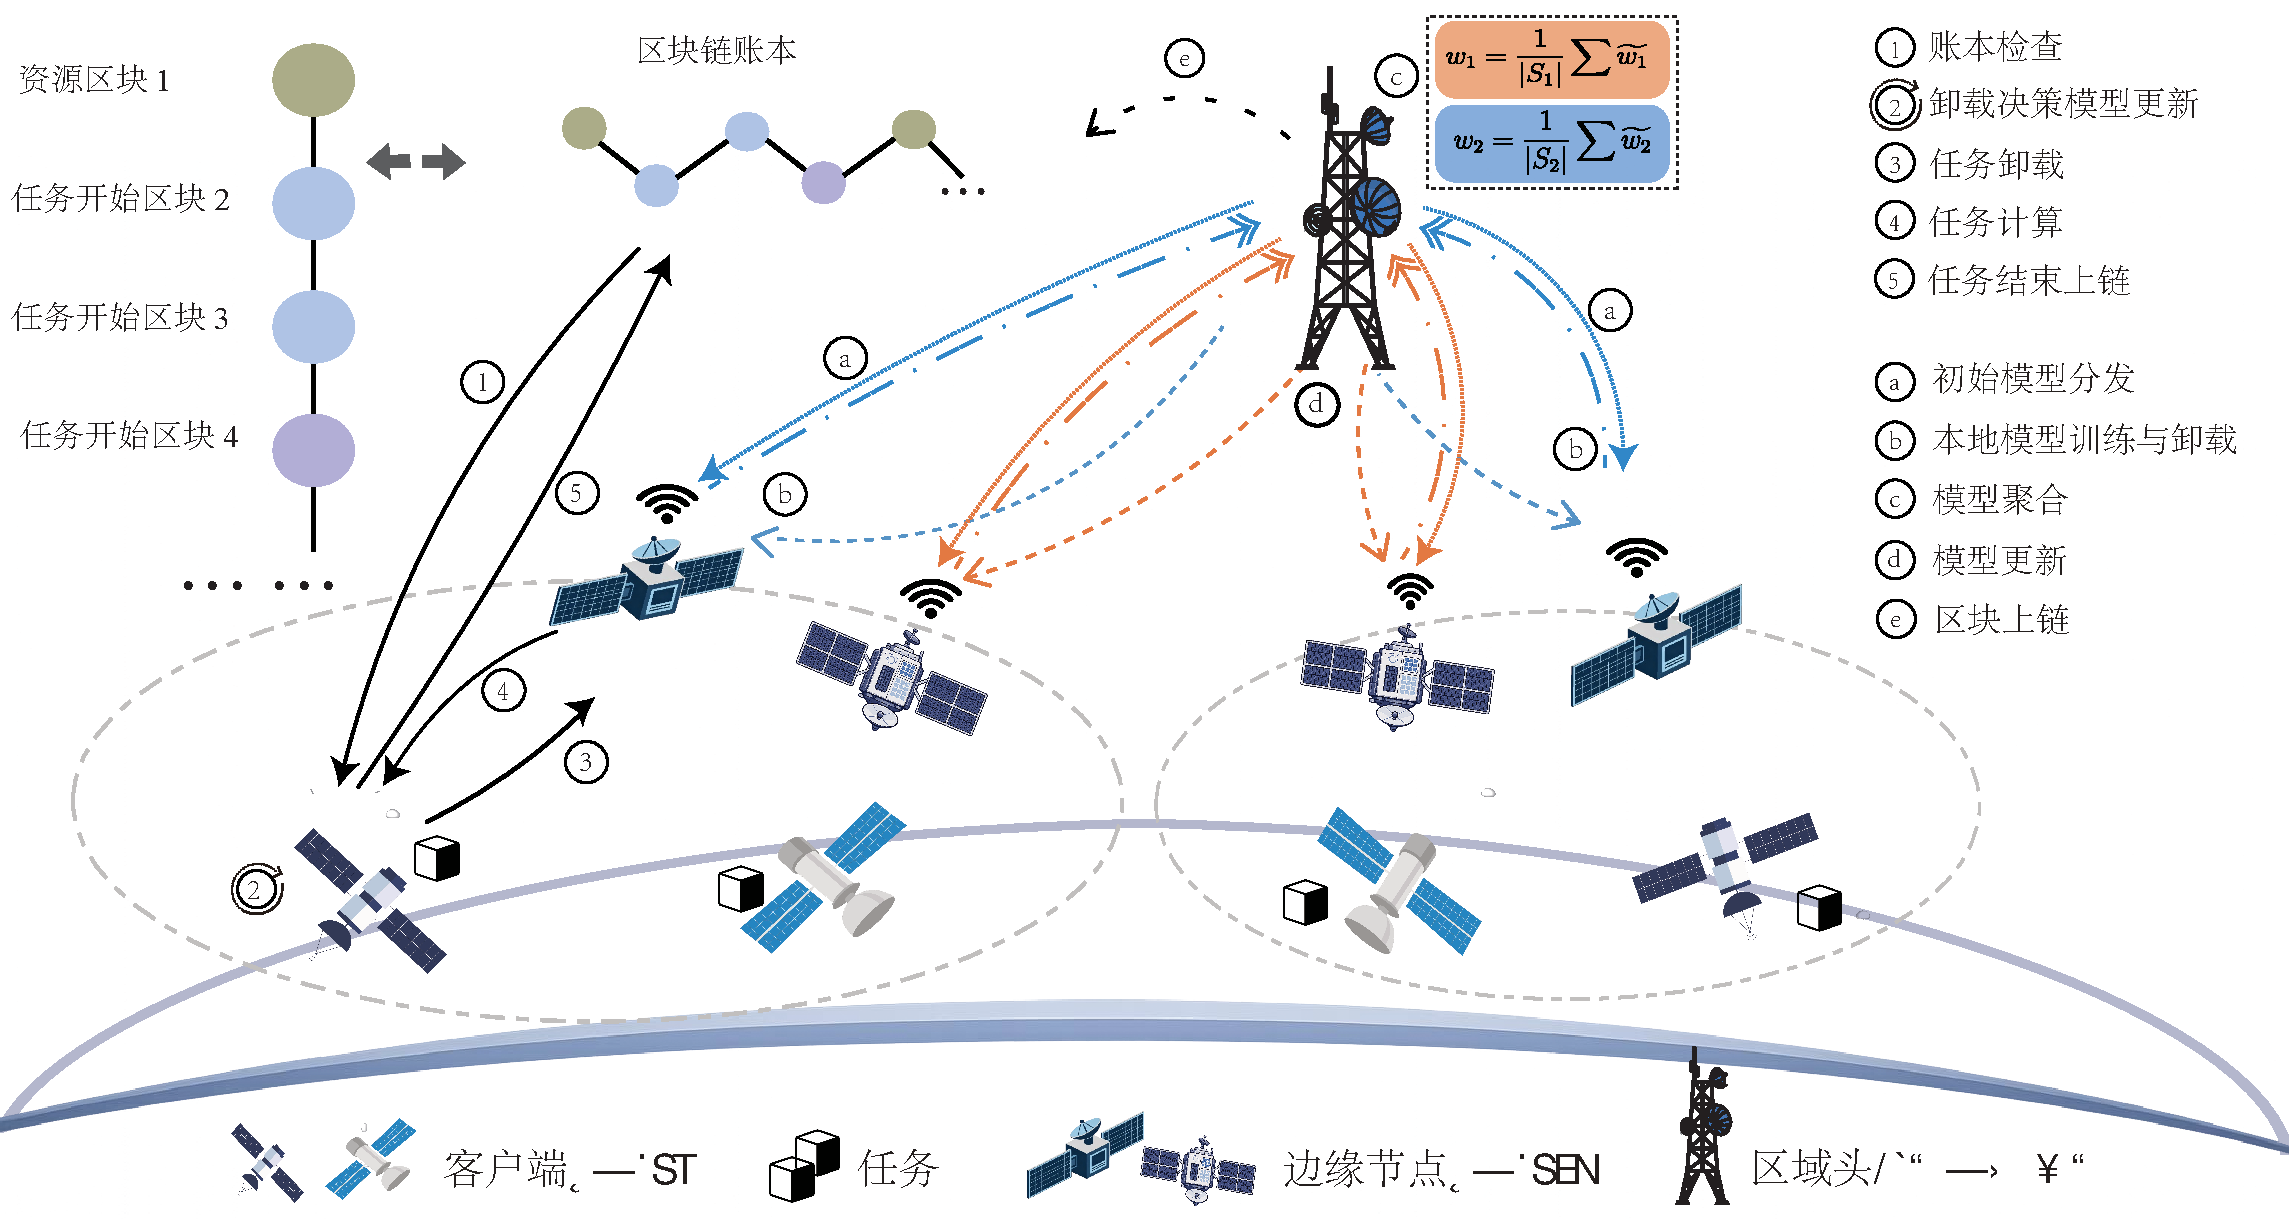
\includegraphics[width=0.95\textwidth]{figures/4-2.pdf}
    \caption{任务级卸载的系统级双时间尺度架构与信息交互流程}
    \label{fig:ch5_system_framework}
\end{figure}

在该结构中，联盟链并不替代终端进行实时卸载决策，而是提供可信但非实时的链上公共摘要和模型版本凭据；联邦协调单元也不直接接管任务执行，而是在后台完成预测模型的簇内聚合与版本维护。表~\ref{tab:ch5_role_division} 总结了任务级卸载框架中的主要参与者及其职责。

\begin{table}[H]
    \centering
    \caption{任务级卸载框架中的角色划分}
    \label{tab:ch5_role_division}
    \begin{tabular}{p{2.5cm}p{8.8cm}}
        \toprule
        角色         & 主要职责                                                 \\
        \midrule
        卫星终端 ST    & 生成新任务、采集本地 CPU/队列/剩余能量状态、读取链上扩展摘要、获得并发开销预测并执行本地/卸载动作 \\
        卫星边缘节点 SEN & 接收外部任务、维护执行队列、反馈任务完成状态、沉淀历史执行日志并参与联邦训练               \\
        联盟链账本      & 维护候选节点摘要、任务开始区块、任务结束区块、模型版本号与哈希摘要，提供异步非实时全局视图        \\
        联邦协调单元     & 根据负载模式进行簇划分、完成簇内聚合与异常更新筛除、下发最新预测模型                   \\
        DQN 决策代理   & 将任务特征、本地状态、链上扩展摘要和预测先验映射为离散卸载动作，并通过经验回放优化策略          \\
        \bottomrule
    \end{tabular}
\end{table}

从任务生命周期看，节点侧卸载决策主要包括以下阶段：1）新任务到达后，终端提取计算量、输入规模、截止期与优先级等属性；2）采样本地资源状态，并从链上公共摘要 $G(t)$ 读取候选节点负载、信誉和账本延迟等状态；3）依据链上模型摘要 $M(t)$ 确认候选目标所属簇及对应预测模型版本；4）调用联邦预测模型估计各候选动作对应的并发开销；5）将任务特征、本地观测、链上扩展摘要和预测先验拼接为状态向量；6）由 DQN 输出本地执行或目标节点卸载动作；7）任务执行结束后，真实时延、能耗、完成状态和模型版本信息继续写入链上记录，为后续状态更新和模型维护提供依据。

\subsection{任务代价模型}

在明确系统组成与卸载流程后，还需要给出节点侧动作选择所依据的任务代价模型。该模型不试图重新求解系统层资源分配，而是面向当前到达任务，分别刻画本地执行与边缘卸载两类动作的时延、能耗以及后续并发扰动来源。

对任意时刻到达终端的一个新任务，记其描述为
\begin{equation}
    T_i = \left(C_i,\, S_i,\, D_i,\, \tau_i,\, \zeta_i \right),
    \label{eq:ch5_task_tuple}
\end{equation}
其中，$C_i$ 表示任务计算量，$S_i$ 表示输入数据大小，$D_i$ 为最大可接受完成时延或截止期，$\tau_i$ 为任务类型编码，$\zeta_i$ 为任务优先级。这里使用 $D_i$ 表示时延约束，是为了避免与任务符号 $T_i$ 发生混淆。

为保持与第\ref{chap:ch3_unified_model}章任务模型的一致性，本章仅在任务层单任务决策视角下调整记号。第\ref{chap:ch3_unified_model}章中的 $T_k=(s_k,c_k,d_k,\tau_k,\zeta_k,t_k^{\mathrm{arr}})$ 强调整体系统中的任务属性和到达时刻；本章中的 $T_i=(C_i,S_i,D_i,\tau_i,\zeta_i)$ 则突出当前到达任务的计算量、输入规模和截止期等决策特征，其中到达时间由当前决策时刻 $t$ 隐含。两章任务符号的对应关系如表~\ref{tab:ch5_task_symbol_mapping} 所示。

\begin{table}[H]
    \centering
    \caption{第三章与第五章任务符号对应关系}
    \label{tab:ch5_task_symbol_mapping}
    \begin{tabular}{p{3.0cm}p{3.0cm}p{5.5cm}}
        \toprule
        第\ref{chap:ch3_unified_model}章符号 & 本章符号       & 含义说明                        \\
        \midrule
        $s_k$                            & $S_i$      & 任务输入数据规模                    \\
        $c_k$                            & $C_i$      & 完成任务所需计算量或 CPU 周期数          \\
        $d_k$                            & $D_i$      & 最大可接受完成时延或截止期               \\
        $\tau_k$                         & $\tau_i$   & 任务类型编码                      \\
        $\zeta_k$                        & $\zeta_i$  & 任务优先级                       \\
        $t_k^{\mathrm{arr}}$             & 当前决策时刻 $t$ & 任务到达时间；在任务层单任务决策中由时刻 $t$ 隐含 \\
        \bottomrule
    \end{tabular}
\end{table}

与第\ref{chap:ch4_system_resource_allocation}章面向较长时间尺度的系统层可信协同不同，本章关注的是{单任务在到达瞬间面临的局部动作选择}。设候选动作集合为
\begin{equation}
    \mathcal{A} = \left\{0,1,2,\ldots,N_c\right\},
    \label{eq:ch5_action_set}
\end{equation}
其中，动作 $0$ 表示本地执行，动作 $n \in \{1,\ldots,N_c\}$ 表示卸载至第 $n$ 个可达候选边缘节点。候选集合并非全网节点集合，而是由第\ref{chap:ch4_system_resource_allocation}章系统层协同资源分配结果、当前链路可达性和信誉阈值共同过滤得到。节点侧决策需要在极短时间窗口内完成，因此策略不仅要追求较低的任务代价，还需要满足在线推理开销约束。

需要强调的是，式\eqref{eq:ch5_action_set} 中的动作是任务层单任务到达瞬间的最终执行动作，其候选节点集合已经受到第\ref{chap:ch4_system_resource_allocation}章系统层输出的任务流向偏好、资源约束和信誉门限限制。换言之，第四章决定“哪些节点在当前系统状态下适合作为候选协同对象”，本章进一步决定“当前具体任务是否本地执行以及卸载至哪个候选节点”。二者分别对应系统层统计窗口内的协同约束和任务层到达瞬间的执行选择。

为支撑后续奖励函数和评价指标设计，本节先给出单任务在本地执行和边缘卸载两种情形下的时延、能耗模型。需要说明的是，本章的时延与能耗表达是在第\ref{chap:ch3_unified_model}章基础执行代价模型上的任务层细化：第\ref{chap:ch3_unified_model}章给出了本地计算、星间传输、远端执行和等待维持能耗的统一形式，本章进一步面向单任务实时卸载，将本地等待期间的空闲维持功耗显式写入本地能耗，并用系数 $\eta_n$ 将候选边缘节点侧执行能耗折算为任务代价。该处理不改变基础模型的物理含义，而是服务于任务层总代价函数和 DQN 奖励反馈的构造。

若任务在本地执行，则其完成时延由本地等待时延和本地计算时延共同构成：
\begin{equation}
    L_i^{\mathrm{loc}}(t) = W_i^{\mathrm{loc}}(t) + \frac{C_i}{f_i^{\mathrm{loc}}(t)},
    \label{eq:ch5_local_delay}
\end{equation}
其中，$W_i^{\mathrm{loc}}(t)$ 表示任务进入本地队列后的等待时间，$f_i^{\mathrm{loc}}(t)$ 为终端在当前时刻可分配给该任务的有效计算频率。相应地，本地执行能耗可写为
\begin{equation}
    E_i^{\mathrm{loc}}(t) = \kappa_i C_i \left( f_i^{\mathrm{loc}}(t) \right)^2
    + P_i^{\mathrm{idle}} W_i^{\mathrm{loc}}(t),
    \label{eq:ch5_local_energy}
\end{equation}
其中，$\kappa_i$ 为设备有效电容系数，$P_i^{\mathrm{idle}}$ 用于近似本地等待期间的空闲维持功耗。若不考虑本地排队或等待能耗，上式可退化为常见的动态功耗模型。

若任务卸载到候选边缘节点 $n$，则其端到端完成时延可分解为上行传输时延、传播时延、边缘基础排队时延、边缘计算时延和并发扰动时延五部分，即
\begin{equation}
    L_i^{\mathrm{off}}(n,t) = \frac{S_i}{R_{i,n}^{\mathrm{up}}(t)} + d_{i,n}^{\mathrm{prop}}(t)
    + W_{n}^{\mathrm{edge}}(t) + \frac{C_i}{F_n(t)} + \Delta_i(n,t),
    \label{eq:ch5_offload_delay}
\end{equation}
其中，$R_{i,n}^{\mathrm{up}}(t)$ 为上行传输速率，$d_{i,n}^{\mathrm{prop}}(t)$ 为传播时延，$W_{n}^{\mathrm{edge}}(t)$ 为不考虑新任务扰动时目标节点已有队列造成的基础等待时间，$F_n(t)$ 为目标节点当前可用计算能力，$\Delta_i(n,t)$ 为将新任务放置到节点 $n$ 后额外产生的并发开销。该写法将“已有队列导致的常规等待”和“新任务加入后造成的资源竞争扰动”分开，有助于后续突出并发开销预测模块的作用。

相应地，卸载能耗可写为
\begin{equation}
    E_i^{\mathrm{off}}(n,t) = P_i^{\mathrm{tx}}\frac{S_i}{R_{i,n}^{\mathrm{up}}(t)}
    + P_i^{\mathrm{idle}}\left(d_{i,n}^{\mathrm{prop}}(t)+W_{n}^{\mathrm{edge}}(t)\right)
    + \eta_n \frac{C_i}{F_n(t)},
    \label{eq:ch5_offload_energy}
\end{equation}
其中，$P_i^{\mathrm{tx}}$ 为终端发射功率，$\eta_n$ 为将目标节点执行能耗折算回任务代价的系数。式~（\ref{eq:ch5_offload_energy}） 不仅刻画了传输能耗，也保留了等待和边缘侧执行的代价信息，从而避免策略一味追求低时延卸载而忽略系统整体能源消耗。进一步地，$\eta_n C_i/F_n(t)$ 可理解为第\ref{chap:ch3_unified_model}章远端执行能耗项在任务层决策中的折算形式；若需要更精细的硬件功耗刻画，也可替换为第\ref{chap:ch3_unified_model}章给出的动态功耗表达。

上述变量具有明确的层次来源。任务计算量、输入数据规模、截止期和优先级来自业务层任务描述；本地 CPU 占用、队列长度、剩余能量和可用频率由终端实时采样获得；候选节点平均负载、负载方差和信誉评分等信息来自第\ref{chap:ch3_unified_model}章定义的链上公共摘要 $G(t)$，模型版本号、模型哈希和所属簇信息来自链上模型摘要 $M(t)$，二者共同构成任务层扩展摘要 $G^{\mathrm{task}}(t)$；执行中任务剩余工作量、上下文切换强度和资源争用统计则由边缘节点日志沉淀，并在联邦训练阶段转化为监督样本。与此同时，式~（\ref{eq:ch5_offload_delay}） 与式~（\ref{eq:ch5_offload_energy}） 建立在以下建模假设之上：其一，任务到达可用泊松流或离散事件过程近似；其二，边缘节点在短时间窗内的标称算力变化相对平缓；其三，链上摘要虽然可能存在陈旧性，但版本顺序和摘要内容具有可信性与可验证性。后续实验中的链上摘要滞后敏感性分析，将进一步讨论上述假设对策略性能的影响。

\subsection{并发开销建模}

传统任务卸载模型通常重点刻画传输时延、排队时延和计算时延，但在候选节点并发执行多个任务时，仅靠这些基础代价仍不足以描述真实卸载后果。并发开销是本章区别于传统卸载模型的关键变量。设在时刻 $t$，目标节点 $n$ 上已有执行中任务集合 $\mathcal{T}_{n}^{\mathrm{exec}}(t)$，新任务 $T_i$ 被放置到该节点后，系统会因 CPU 时间片争用、缓存冲突、内存带宽竞争和 I/O 排队而出现额外时延。为了同时刻画新任务自身被拖慢和存量任务被扰动两类影响，将任务 $T_i$ 产生的并发开销定义为
\begin{equation}
    CO_i(n,t) =
    \left[L_i^{\mathrm{conc}}(n,t)-L_i^{\mathrm{base}}(n,t)\right]
    + \sum_{e \in \mathcal{T}_{n}^{\mathrm{exec}}(t)}
    \left[\widetilde{L}_{e}^{\mathrm{conc}}(n,t)-\widetilde{L}_{e}^{\mathrm{base}}(n,t)\right],
    \label{eq:ch5_co_formal}
\end{equation}
其中，$L_i^{\mathrm{base}}(n,t)$ 表示新任务在目标节点不受额外并发扰动时的基准完成时延，$L_i^{\mathrm{conc}}(n,t)$ 表示新任务加入真实并发环境后的完成时延；$\widetilde{L}_{e}^{\mathrm{base}}(n,t)$ 表示存量任务 $e$ 在没有新任务 $T_i$ 加入时的预计剩余完成时延，$\widetilde{L}_{e}^{\mathrm{conc}}(n,t)$ 表示新任务加入后该存量任务的剩余完成时延。与只关注新任务自身时延的定义相比，式~（\ref{eq:ch5_co_formal}） 同时计入了新任务进入成本与存量任务受扰成本，因此更符合节点侧真实的资源竞争机制。为避免符号混淆，后文中 $CO_i(n,t)$ 用作并发开销的完整定义，$\Delta_i(n,t)$ 表示进入时延模型和总代价函数的并发扰动项，$\widehat{\Delta}_i(n,t)$ 表示联邦预测模型给出的估计值。

图~\ref{fig:ch5_co_illustration} 展示了并发开销的形成机理。该图应与式~（\ref{eq:ch5_co_formal}） 对应理解：左侧表示无新任务加入时存量任务按相对稳定的资源份额推进；右侧表示新任务进入后，CPU、Cache、Memory 和 I/O 等共享资源被重新分配，存量任务出现受扰延迟，新任务也因竞争产生额外等待。因而，并发开销不是单个任务的固定附加项，而是由任务组合、资源瓶颈和执行上下文共同决定的耦合代价。

\begin{figure}[H]
    \centering
    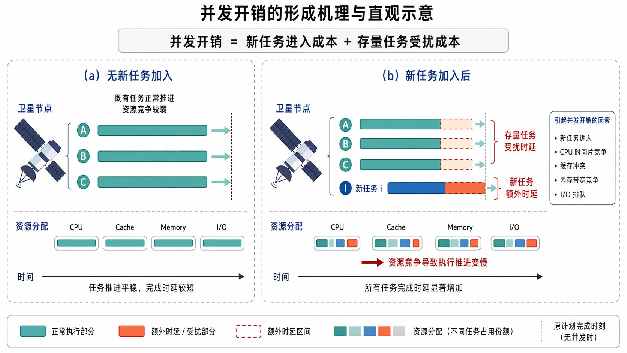
\includegraphics[width=0.92\textwidth]{figures/4-3.pdf}
    \caption{并发开销的形成机理与资源争用示意}
    \label{fig:ch5_co_illustration}
\end{figure}

在实现过程中，式~（\ref{eq:ch5_co_formal}） 所涉及的未来并发时延难以在决策瞬间直接获得，因此还需构造一个可学习、可预测的近似表达。记目标节点当前并发任务数为 $k_n(t)$，节点当前可用计算能力为 $F_n(t)$，执行中任务 $e$ 的剩余计算量为 $C_e^{\mathrm{rem}}(t)$，并用 $\chi_{i,e}\in[0,1]$ 表示新任务与存量任务在资源需求类型上的竞争强度，则并发扰动可近似写为
\begin{equation}
    \Delta_i(n,t) \approx \frac{\left(k_n(t)-1\right)C_i}{F_n(t)}
    + \sum_{e \in \mathcal{T}_{n}^{\mathrm{exec}}(t)}
    \frac{\chi_{i,e} C_e^{\mathrm{rem}}(t)}{F_n(t)},
    \label{eq:ch5_co_approx}
\end{equation}
该表达式揭示了并发开销与新任务计算量、当前并发任务数、存量任务剩余工作量以及任务间资源竞争强度之间的正相关关系，便于在后续样本标注、特征选择和模型解释中使用。当缺少细粒度资源画像时，可令 $\chi_{i,e}=1$ 得到保守估计。

从统计学习角度可以将并发开销写为
\begin{equation}
    CO_i(n,t) \approx F_{\mathrm{new}}(T_i,n,\mathrm{obs})
    + G_{\mathrm{exec}}(\mathcal{T}_{n}^{\mathrm{exec}}(t),n,\mathrm{obs})
    + R_i(n,t),
    \label{eq:ch5_co_decomp}
\end{equation}
其中，$F_{\mathrm{new}}(\cdot)$ 捕获新任务加入带来的瞬时冲击，$G_{\mathrm{exec}}(\cdot)$ 刻画已执行任务间的持续资源竞争，$R_i(n,t)$ 表示未建模的高阶耦合残差。该可分解表达虽不直接用于在线推理，却有助于解释为何联邦模型在轻负载和重负载场景下会表现出不同的误差模式：前者更依赖新任务特征，后者更依赖存量任务组合和运行背景。

考虑时延、能耗和并发扰动三类代价，本章将动作 $a_t$ 对应的单任务总代价定义为
\begin{equation}
    J_i(a_t) = \omega_L L_i(a_t) + \omega_E E_i(a_t) + \omega_C \Delta_i(a_t),
    \qquad
    \omega_L+\omega_E+\omega_C=1,
    \label{eq:ch5_total_cost}
\end{equation}
其中，$L_i(a_t)$ 为动作执行后的端到端完成时延，$E_i(a_t)$ 为对应能耗，$\Delta_i(a_t)$ 表示动作引起的并发扰动；对于本地执行动作，可令 $\Delta_i(a_t)$ 表示本地队列中存量任务受到的额外扰动，也可在只关注边缘并发时取零。三个权重参数可根据业务偏好灵活调整：对实时业务可提高 $\omega_L$，对能源敏感任务可提高 $\omega_E$，对高拥塞控制场景则可适当增加 $\omega_C$。采用 $\omega$ 作为代价权重，是为了避免与后续 DQN 中的折扣因子符号混用。

式~（\ref{eq:ch5_total_cost}） 的意义并不仅在于给出加权求和目标，更重要的是为后续 DQN 奖励函数设计提供统一的任务层优化视角。第\ref{chap:ch4_system_resource_allocation}章关注较长时间尺度下的系统层协同资源分配，本章则将优化边界收缩到{节点侧单任务决策}，从而在保持跨层方法链连贯性的同时，避免重复求解上一章已经讨论过的系统层资源协同问题。

\subsection{状态表征与 MDP 建模}

为了使并发开销能够被机器学习模型预测，并使 DQN 能够进行可执行的在线决策，需要构造一个统一的复合状态表征。设可观测特征向量为
\begin{equation}
    \bm{x} = \left[ \bm{x}^{\mathrm{task}},\,
        \bm{x}^{\mathrm{local}},\,
        \bm{x}^{\mathrm{chain}},\,
        \bm{x}^{\mathrm{conc}}
        \right],
    \label{eq:ch5_feature_vector}
\end{equation}
其中：
\begin{itemize}[leftmargin=2.5em]
    \item $\bm{x}^{\mathrm{task}}$：新任务特征，包括计算量、输入大小、时延阈值、任务类型编码、优先级等；
    \item $\bm{x}^{\mathrm{local}}$：本地状态，包括本地 CPU 占用、队列长度、剩余能量、可用频率和链路质量估计等；
    \item $\bm{x}^{\mathrm{chain}}$：链上公共摘要 $G(t)$ 的任务层相关分量，包括候选节点平均负载、负载方差、信誉评分、账本确认延迟估计等；
    \item $\bm{x}^{\mathrm{conc}}$：并发环境统计，包括目标节点当前并发任务数、执行中任务总剩余工作量、平均内存占用和上下文切换强度等。
\end{itemize}

所有连续特征在进入模型前都进行标准化处理，即
\begin{equation}
    \tilde{x}_j = \frac{x_j - \mu_j}{\sigma_j + \varepsilon},
    \label{eq:ch5_normalize}
\end{equation}
其中，$\mu_j$ 和 $\sigma_j$ 分别为训练集统计均值和标准差，$\varepsilon$ 为数值稳定常数。

节点侧观测天然不完全：本地节点只能直接观测自身状态，难以获取其他候选节点的细粒度实时轨迹；链上公共摘要虽然提供一致且可追溯的系统级视图，时间戳却可能早于当前决策时刻。因此，本章卸载问题本质上是部分可观测、带滞后信息的序贯决策问题。引入 FL 预测模块的意义，正在于利用历史数据学习并发风险先验，在缺乏完整实时信息的条件下补充节点侧观测。

在上述状态表征基础上，节点侧任务卸载进一步被建模为马尔可夫决策过程
\begin{equation}
    \mathcal{M} = \langle \mathcal{S}, \mathcal{A}, \mathcal{P}, \mathcal{R} \rangle.
\end{equation}
其中：
\begin{itemize}[leftmargin=2.5em]
    \item 状态空间 $\mathcal{S}$ 由任务特征、本地资源状态、链上扩展摘要和 FL 预测值共同组成；
    \item 动作空间 $\mathcal{A}$ 为“本地执行 + 若干候选 SEN”构成的离散集合；
    \item 状态转移概率 $\mathcal{P}$ 由任务到达、链路变化、资源占用演化和预测结果更新共同决定；
    \item 奖励函数 $\mathcal{R}$ 采用总代价负值并叠加轻量奖惩项。
\end{itemize}

严格而言，该过程具有部分可观测特征。本文将本地观测、链上扩展摘要和预测先验拼接为扩展状态，并以该扩展状态近似满足马尔可夫性，从而采用 DQN 进行求解。

考虑到任务层在线推理的时延约束，本章选择基于离散动作值函数的 DQN，而非连续动作策略梯度方法。本场景的动作集合有限，DQN 具有较高的推理效率和较低的实现复杂度；同时，将主要模型复杂度集中于并发开销预测环节，比在在线决策阶段引入更复杂的连续动作网络更符合本章的问题结构。

\section{并发开销预测方法}
\label{sec:ch5_fl_prediction}
第~5.2 节已经说明并发开销为何会影响任务层卸载质量。本节进一步回答如何学习这一隐藏变量。并发开销虽然可以通过历史执行日志标注，但这些日志分散在不同 SEN 上，并包含任务类型、执行轨迹和资源占用等敏感信息；若集中上传，通信和隐私代价较高；若各节点只依赖本地样本，又容易因样本规模有限和数据分布偏置导致预测不稳定。为此，本节采用聚类联邦学习，在不上传原始日志的前提下，使负载模式相近的节点共享模型能力。

\subsection{预测目标与样本构造}

并发开销预测本质上是一个监督回归问题。其输入为式~（\ref{eq:ch5_feature_vector}） 定义的多维特征，输出为目标节点在接受新任务后的并发开销估计值 $\widehat{\Delta}$ 及其不确定性信息。设节点本地构造的监督样本为
\begin{equation}
    \mathcal{D}_k = \left\{ \left(\bm{x}^{(m)}, y^{(m)} \right) \right\}_{m=1}^{N_k},
\end{equation}
其中，$y^{(m)}$ 为根据运行日志标注得到的真实并发开销。对于每个样本，需要记录任务到达前后的队列长度、CPU 频率、内存占用、任务开始时间、完成时间、输入大小、计算量等信息，再依照式~（\ref{eq:ch5_co_formal}） 或式~（\ref{eq:ch5_co_approx}） 计算标签。

为了使预测模型尽可能覆盖多样化的竞争形态，本章采用“双代理负载”的思路：一类是图像处理任务，用于模拟视觉感知类边缘业务；另一类是数值计算任务，用于模拟计算密集但数据规模较小的负载。这种设计的好处在于，既能让模型观察到数据搬移开销与计算开销同时占优的混合场景，又能避免训练集完全偏向单一类型任务而失去泛化性。

\subsection{预测模型设计}

考虑到输入特征既包含结构化统计量，也可能包含短时间窗内的序列信息，本章在模型结构上兼容两类实现：

\begin{enumerate}[label=\arabic*)]
    \item {MLP 结构}：适用于结构化向量输入。模型通常由 3--5 个全连接隐藏层构成，每层采用 ReLU 激活并可结合 Dropout 抑制过拟合；
    \item {1D-CNN 结构}：当输入拼接了过去若干时间步的 CPU 利用率、队列长度或链路质量序列时，1D-CNN 可以提取时序局部模式，再通过全连接层输出最终预测值。
\end{enumerate}

为了使预测结果能够在决策阶段发挥更稳健的作用，本章采用{均值 + 方差双输出}的设计，即网络输出
\begin{equation}
    f_{\theta}(\bm{x}) = \left(\widehat{\Delta},\, \widehat{\sigma}^2 \right),
\end{equation}
其中，$\widehat{\Delta}$ 为并发开销点估计，$\widehat{\sigma}^2$ 为预测方差估计。增加不确定性分支后，DQN 状态空间中能够带入“模型对该预测是否有把握”的额外信息；在高异构、弱覆盖的样本区间内，不确定性也提醒策略不要过度依赖单一预测值。

预测器本身不追求过深或过重的网络结构，而强调对结构化特征、短时间窗统计序列和不确定性信息的统一表达。本章关心的是“并发开销感知如何服务任务级决策”，模型结构因此保留轻量、可部署和可解释的设计原则，并不把网络复杂度本身列为创新点。

在损失函数设计上，若仅关注点估计，可使用均方误差
\begin{equation}
    \mathcal{L}_{\mathrm{MSE}} = \frac{1}{N}\sum_{m=1}^{N}
    \left( \widehat{\Delta}^{(m)} - \Delta^{(m)} \right)^2.
    \label{eq:ch5_mse_loss}
\end{equation}
若同时训练不确定性分支，则可以采用异方差高斯负对数似然形式
\begin{equation}
    \mathcal{L}_{\mathrm{pred}}
    =
    \frac{1}{N}
    \sum_{m=1}^{N}
    \left[
        \frac{\left(\widehat{\Delta}^{(m)}-\Delta^{(m)}\right)^2}{2\widehat{\sigma}^{2(m)}}
        +
        \frac{1}{2}\log \widehat{\sigma}^{2(m)}
        \right].
    \label{eq:ch5_hetero_loss}
\end{equation}
该损失函数允许模型在噪声较大的区域给出更高的不确定性估计，从而避免对本就难以准确预测的样本过度拟合。

\subsection{聚类联邦训练}

不同边缘卫星节点的本地样本分布具有显著 Non-IID 特征：高性能节点可能长期承载视觉类任务，资源受限节点则更多面对轻量计算或转发类任务。若直接使用统一 FedAvg 训练单一全局模型，模型往往难以兼顾不同簇之间的局部负载模式。基于此，本文采用聚类式联邦学习（clustered FL）对预测模型进行训练。其核心思路是：不再假设全网节点共享同一个最优模型，而是先根据节点负载模式、硬件能力或更新方向将其划分为多个簇，再在簇内执行模型聚合。

面向天基网络的层次化结构，本章将联邦预测框架设计为“全局协调层—区域聚合层—本地训练层”三层架构。与参考章节中“系统组成—工作流程—算法设计”的写法一致，这里先说明各层角色，再给出训练流程与簇内聚合规则。

三层架构的职责分工如表~\ref{tab:ch5_fl_roles} 所示。

\begin{table}[H]
    \centering
    \caption{分层聚类联邦学习架构中的角色划分}
    \label{tab:ch5_fl_roles}
    \begin{tabular}{p{2.7cm}p{3.0cm}p{6.0cm}}
        \toprule
        层级    & 典型实体           & 主要职责                           \\
        \midrule
        全局协调层 & 地面控制中心 / 星座控制器 & 模型版本管理、训练轮次调度、簇级模型下发、链上摘要维护    \\
        区域聚合层 & 核心边缘卫星节点       & 区域内节点分组、异常更新检测、簇内参数加权聚合        \\
        本地训练层 & 参与训练的 SEN 集合   & 基于本地执行日志训练预测模型，不上传原始样本，仅上传模型更新 \\
        \bottomrule
    \end{tabular}
\end{table}

在一次完整的联邦训练周期内，预测模型的工作流程可以概括为：1）全局协调层根据节点历史负载模式完成簇划分并下发初始化模型；2）本地训练层在各自执行日志上完成若干轮本地更新；3）区域聚合层对上传参数执行一致性检查、异常更新筛除与簇内加权聚合；4）聚合后的模型版本号和参数哈希写入联盟链，供后续在线推理时进行版本校验与追溯；5）最新簇模型再次下发至簇内节点，进入下一轮训练。上述流程使预测模型的训练、维护和可信存证形成统一流程。

设第 $c$ 个簇内包含若干节点集合 $C_c$，第 $t$ 轮通信后簇模型参数更新为
\begin{equation}
    \theta_c^{(t+1)} =
    \sum_{k \in C_c}
    \frac{n_k}{\sum_{j \in C_c}n_j}
    \theta_k^{(t+1)},
    \label{eq:ch5_cluster_fedavg}
\end{equation}
其中，$n_k$ 为节点 $k$ 的本地样本量，$\theta_k^{(t+1)}$ 为节点本地更新后的参数。与传统 FedAvg 相比，式~（\ref{eq:ch5_cluster_fedavg}） 的改进并不体现在加权形式本身，而在于聚合只在“样本分布相近的节点簇内”进行，因此更容易捕捉局部任务模式。

在实现层面，聚类式联邦训练不仅是将 FedAvg 改为簇内聚合，还需要与区块链可信控制平面形成一致的状态维护关系。具体而言，区域聚合层在每轮簇内聚合后，可将模型版本号、参数哈希和训练轮次摘要写入联盟链，形成第\ref{chap:ch3_unified_model}章中模型摘要 $M(t)$ 的具体内容，用于模型溯源、版本一致性校验与异常更新留痕；终端节点在调用预测器时只需读取候选节点当前所属簇的最新可用模型版本，从而避免在在线阶段访问原始训练日志。这样的设计使“数据不出域”和“模型可追溯”同时成立，也使预测模块能够自然嵌入前文建立的可信状态体系。

聚类式联邦学习的一个完整训练轮次可由算法~\ref{alg:ch5_clusterfedavg} 概括。相较原始 FedAvg，该流程新增了簇内聚合、异常更新筛查与链上存证三个关键步骤，因此更适合 Non-IID 且可信要求较高的天基边缘场景。

\begin{algorithm}[H]
    \caption{聚类式联邦学习（Clustered FedAvg）训练流程}
    \label{alg:ch5_clusterfedavg}
    \small
    \begin{algorithmic}[1]
        \Statex {输入：}簇划分集合 $\{C_1,\ldots,C_K\}$，本地数据集 $\mathcal{D}_k$，本地训练轮数 $E$，通信轮数 $T$。
        \Statex {输出：}各簇最终预测模型参数 $\theta_c^{(T)}$。
        \For{每个簇 $C_c$}
        \State 初始化簇模型参数 $\theta_c^{(0)}$ 并下发至簇内节点
        \EndFor
        \For{$t=0,1,\ldots,T-1$}
        \For{每个簇 $C_c$ 并行执行}
        \For{每个参与节点 $k\in C_c$}
        \State 以 $\theta_c^{(t)}$ 为初值，在 $\mathcal{D}_k$ 上执行 $E$ 个 epoch 本地更新
        \State 得到本地参数 $\theta_k^{(t+1)}$ 及样本量 $n_k$
        \EndFor
        \State 区域聚合层对上传更新做一致性检查与异常筛除
        \State 按式~(\ref{eq:ch5_cluster_fedavg}) 聚合得到新的簇模型 $\theta_c^{(t+1)}$
        \State 将模型版本号、参数哈希及训练轮次摘要写入联盟链
        \EndFor
        \EndFor
    \end{algorithmic}
\end{algorithm}

在线推理阶段，终端节点并不直接参与联邦训练，而是在需要决策时调用候选边缘节点所属簇的最新预测模型，对每个候选动作的并发开销进行快速估计。这一点十分重要：联邦学习的高开销发生在离线训练或后台异步更新阶段，而在线阶段保留下来的只是一个轻量前向推理过程，因此不会破坏节点侧决策的实时性要求。

\subsection{模型可信维护}

设单个本地预测模型包含 $P_f$ 个参数、每轮训练使用 $B_f$ 个 mini-batch，则节点单轮本地训练复杂度约为 $\mathcal{O}(B_f P_f)$，簇内聚合本质是参数加权求和、复杂度为 $\mathcal{O}(|C_c|P_f)$。聚类式 FL 把全局聚合拆解为若干簇内聚合，单轮同步对全网连通性的要求因此低于统一 FedAvg。在线阶段只保留一次前向推理，预测模块部署时的主要成本不在计算本身，而在模型版本刷新与链上摘要读取的调度。

通信开销上，联邦学习阶段只需在节点与聚合层之间传递参数摘要，无需传输原始日志，“模型移动而非数据移动”在带宽受限、链路可用性波动的天基环境中收益明显；区域聚合层则把大规模全局同步进一步拆为局部同步，降低对全网连通性的苛刻要求。

把模型可信维护纳入考虑后，每轮额外链上开销主要来自模型哈希写入和版本确认，这部分复杂度与模型参数规模无关，只取决于摘要长度和交易确认时延。也就是说，区块链不会显著增加训练算力负担，但会通过信息年龄影响在线可用模型版本的新鲜度。后续实验中的“链上确认延迟敏感性”正是针对这一约束的量化验证。

\section{FL-DQN 卸载决策算法}
\label{sec:ch5_dqn_policy}
并发开销预测本身并不是任务层卸载的最终目标。预测模型只回答“某个候选动作可能带来多大额外扰动”，而节点仍需在本地执行和多个候选卸载目标之间做出离散选择。为此，本节将预测值及其不确定性作为扩展状态输入 DQN，使策略能够在当前任务特征、本地状态、链上摘要和预测先验之间进行综合权衡。

\subsection{状态、动作与奖励}

在获得并发开销预测能力后，节点侧还需解决“面对新任务应当本地执行还是卸载到哪个候选节点”的决策问题。本文将单个 ST 的卸载过程建模为 MDP，其状态向量定义为
\begin{equation}
    s_t =
    \left[
        s_t^{\mathrm{task}},\,
        s_t^{\mathrm{local}},\,
        s_t^{\mathrm{chain}},\,
        s_t^{\mathrm{FL}}
        \right],
    \label{eq:ch5_dqn_state}
\end{equation}
其中，$s_t^{\mathrm{task}}$ 包含任务计算量、数据规模、截止期、任务类型编码与优先级；$s_t^{\mathrm{local}}$ 包含本地 CPU 占用、队列长度、剩余能量与链路质量估计；$s_t^{\mathrm{chain}}$ 来自链上公共摘要 $G(t)$ 中的候选节点状态；$s_t^{\mathrm{FL}}$ 则由并发开销预测模型给出，包括各候选动作的 $\widehat{\Delta}_i(n,t)$ 及其不确定性 $\widehat{\sigma}_i^2(n,t)$。模型版本号、模型哈希和所属簇信息由模型摘要 $M(t)$ 提供，主要用于确定预测模型版本与适用范围。实际部署中，候选节点数量会随链路可达性变化。本文设定最大候选数 $N_c^{\max}$：当实际候选数不足时采用零填充并设置动作掩码，当候选数超过上限时根据信誉、链路质量和基础负载筛选前 $N_c^{\max}$ 个候选节点，从而保持 DQN 输入输出维度固定。

表~\ref{tab:ch5_state_space} 总结了复合状态空间的设计。

\begin{table}[H]
    \centering
    \caption{节点侧决策的复合状态空间设计}
    \label{tab:ch5_state_space}
    \begin{tabular}{p{3.1cm}p{5.8cm}p{3.0cm}}
        \toprule
        状态分量          & 主要内容                               & 作用              \\
        \midrule
        任务特征向量        & 任务计算量、输入数据大小、截止期、任务类型编码、优先级        & 刻画当前任务需求        \\
        本地资源与链路状态     & 本地 CPU 占用、队列长度、剩余能量、可用频率、链路时延与带宽估计 & 反映当前本地资源与通信条件   \\
        链上公共摘要 $G(t)$ & 候选节点平均负载、负载方差、信誉评分、账本延迟估计          & 提供可信但非实时的系统级上下文 \\
        FL 预测先验       & 各候选动作的并发开销预测值与不确定性                 & 显式表征卸载后的额外风险    \\
        \bottomrule
    \end{tabular}
\end{table}

奖励函数在总代价负值的基础上引入轻量奖惩机制：
\begin{equation}
    r_t = -\left(
    \omega_L L_i^{\mathrm{obs}}
    + \omega_E E_i^{\mathrm{obs}}
    + \omega_C \Delta_i^{\mathrm{obs}}
    \right)
    - \lambda_b P_{\mathrm{imbalance}}
    - \lambda_u \overline{\sigma}_t
    + R_{\mathrm{succ}},
    \label{eq:ch5_reward}
\end{equation}
其中，$L_i^{\mathrm{obs}}$、$E_i^{\mathrm{obs}}$ 和 $\Delta_i^{\mathrm{obs}}$ 分别表示任务执行后观测到的真实时延、能耗和并发扰动；$P_{\mathrm{imbalance}}$ 表示负载不均衡惩罚项，用于抑制任务长期集中到少数高性能边缘节点；$\overline{\sigma}_t$ 表示当前被选动作或候选动作集合上的平均预测不确定性，用于避免策略在高不确定区域过度激进；$R_{\mathrm{succ}}$ 为任务在截止期内完成、满足优先级约束或成功避开高拥塞节点时给予的正向奖励。由于 $\Delta_i^{\mathrm{obs}}$ 只有在任务完成后才能准确计算，在线训练时采用两阶段奖励更新：动作执行后先根据 $\widehat{\Delta}_i$ 给出临时塑形奖励，任务结束后再用观测到的真实并发扰动修正对应经验样本。这样既保留了预测先验对动作选择的前瞻作用，又避免把预测值误认为最终真实奖励。

FL 预测先验在机制上同时承担两类作用——作为扩展状态的一部分，它帮助智能体在动作选择前识别潜在拥塞；作为奖励塑形与不确定性惩罚的输入，它在候选节点当前负载相近但未来并发开销不同时，引导策略选择更低风险的动作。再加上 $P_{\mathrm{imbalance}}$ 的负载均衡约束，策略不再只追求单次动作收益，而能够兼顾较长时间尺度上的节点利用均衡。

\subsection{Q 网络训练}

由于动作空间是有限离散集合，本文采用 DQN 学习最优动作价值函数 $Q^*(s,a)$。令主网络参数为 $\theta_q$，目标网络参数为 $\theta_q^{-}$，DQN 的 Bellman 目标值写为
\begin{equation}
    y_t =
    r_t + \rho \max_{a'} Q(s_{t+1},a';\theta_q^-),
    \label{eq:ch5_bellman_target}
\end{equation}
损失函数为
\begin{equation}
    \mathcal{L}_{\mathrm{DQN}}(\theta_q) =
    \mathbb{E}_{(s_t,a_t,r_t,s_{t+1}) \sim \mathcal{B}}
    \left[
        \left(
        y_t - Q(s_t,a_t;\theta_q)
        \right)^2
        \right],
    \label{eq:ch5_dqn_loss}
\end{equation}
其中，$\mathcal{B}$ 为经验回放池，$\rho\in[0,1)$ 为折扣因子。这里将折扣因子记为 $\rho$，以避免与式~（\ref{eq:ch5_total_cost}） 中的代价权重混淆。

为提高训练稳定性，本章沿用标准 DQN 的三项关键机制：

\begin{enumerate}[label=\arabic*)]
    \item {经验回放}：将交互产生的样本打乱后重用，削弱序列相关性；
    \item {目标网络}：使用滞后更新的目标网络生成目标值，减少训练震荡；
    \item {$\varepsilon$-greedy 探索}：在探索与利用之间进行平衡，防止策略过早陷入局部最优。
\end{enumerate}

在网络结构上，考虑到状态维度相对有限且要求在线推理足够快，本文使用两层或三层全连接网络逼近 $Q(s,a;\theta)$，隐藏层采用 ReLU 激活。相比于更复杂的 dueling、double 或 attention 结构，这种配置在节点侧具有更低的实现门槛和推理开销，更符合“轻量快速决策”的系统定位。当然，在实验中我们仍保留增强型 DQN 变体作为对比基线，以检验“改进 DRL 结构”和“引入预测先验”两条路线的相对收益。

\subsection{在线决策流程}

本章的关键并非单独提出联邦预测器或单独训练一个 DQN，而是把这两者衔接起来。与图~\ref{fig:ch5_system_framework} 强调“系统级双时间尺度架构”不同，图~\ref{fig:ch5_closed_loop} 聚焦于单任务到达瞬间的节点侧在线决策过程：节点收集本地状态、链上公共摘要与模型摘要后，调用对应簇的最新预测模型生成各候选动作的并发开销估计与不确定性，把它们与原始状态一同送入 DQN；DQN 输出动作执行后，环境返回的时延、能耗与任务结果以奖励形式回流，驱动后续的策略更新。

\begin{figure}[H]
    \centering
    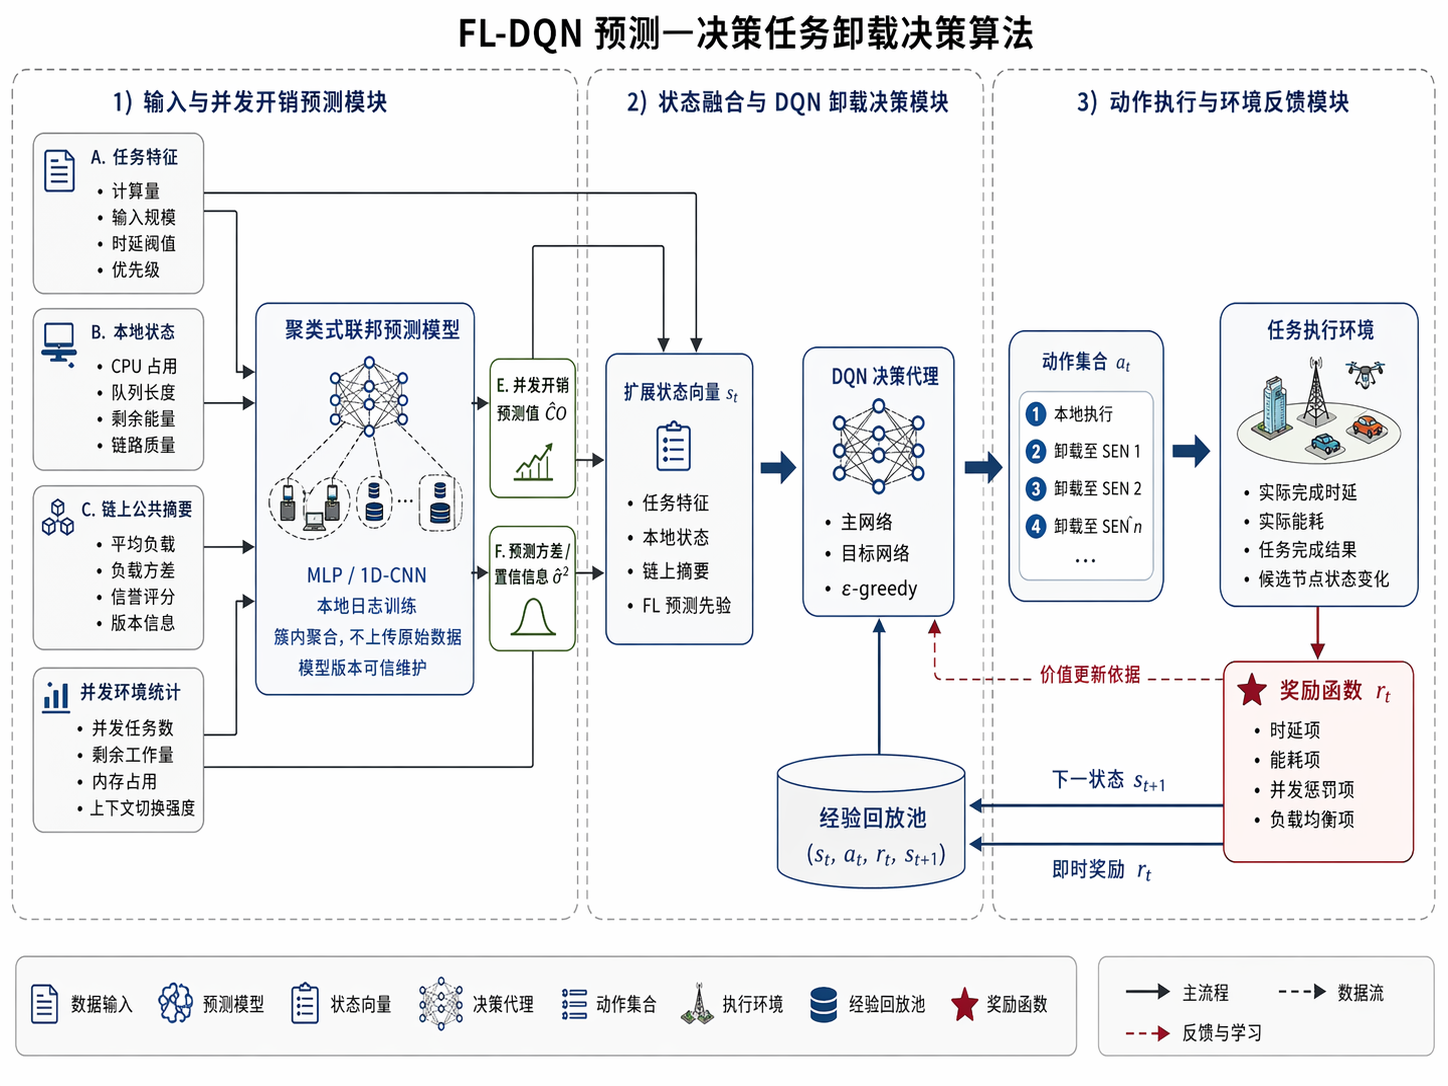
\includegraphics[width=0.96\textwidth]{figures/4-5.png}
    \caption{融合并发开销预测先验的 FL-DQN 在线卸载决策流程}
    \label{fig:ch5_closed_loop}
\end{figure}

这种衔接的价值在于，它把难以编入解析策略的“未来并发开销”显式注入到了决策模块——DQN 此时不是在即时观测上做反应式决策，而是在带预测先验的扩展状态上做前瞻式决策。在高并发或链上摘要滞后的工况下，这种差异通常会反映为更平缓的时延退化斜率和更好的系统鲁棒性。

完整的在线流程整理为表~\ref{tab:ch5_online_policy} 所列的七个步骤。

\begin{table}[H]
    \centering
    \caption{FL-DQN 在线卸载决策流程}
    \label{tab:ch5_online_policy}
    \begin{tabular}{p{1.0cm}p{11.2cm}}
        \toprule
        步骤 & 流程描述                                                                              \\
        \midrule
        1  & 终端节点接收新任务，提取计算量、数据大小、任务类型、优先级和截止期等特征。                                             \\
        2  & 从本地环境读取 CPU、内存、队列长度、剩余能量与链路状态，从链上公共摘要 $G(t)$ 中获取候选边缘节点状态，并根据模型摘要 $M(t)$ 确认预测模型版本。 \\
        3  & 按候选目标节点所属簇调用联邦预测模型，对各候选动作的并发开销和预测不确定性进行快速推理。                                      \\
        4  & 将任务特征、本地资源状态、链上扩展摘要和预测先验拼接为状态向量 $s_t$。                                            \\
        5  & DQN 计算各动作的 $Q$ 值，并按 $\varepsilon$-greedy 规则选择本地执行或目标节点卸载动作。                       \\
        6  & 环境返回任务完成时延、能耗、并发扰动和完成结果，据此计算奖励并写入经验回放池。                                           \\
        7  & 主网络按 mini-batch 更新参数，目标网络按固定步长同步；策略持续与环境交互直至收敛。                                   \\
        \bottomrule
    \end{tabular}
\end{table}

为了更清楚地展示“预测先验如何进入在线动作选择”，算法~\ref{alg:ch5_fldqn_online} 对 FL-DQN 的节点侧执行流程给出伪代码描述。该伪代码与图~\ref{fig:ch5_closed_loop} 的区别在于：前者强调实现时的控制流，后者强调预测与决策之间的信息关系。

\begin{algorithm}[H]
    \caption{FL-DQN 在线任务卸载决策流程}
    \label{alg:ch5_fldqn_online}
    \small
    \begin{algorithmic}[1]
        \Statex {输入：}最新可用联邦预测模型 $f_{\theta_f}$，DQN 主网络 $Q(\cdot;\theta_q)$，目标网络 $Q(\cdot;\theta_q^-)$，经验回放池 $\mathcal{B}$。
        \Statex {输出：}收敛后的节点侧卸载策略。
        \For{每个决策周期}
        \State 接收新任务并提取任务特征、本地资源状态与链上扩展摘要
        \For{每个候选动作 $a\in\mathcal{A}$}
        \State 构造动作相关特征向量 $\bm{x}(s_t,a)$
        \State 调用 $f_{\theta_f}$ 得到并发开销预测值及不确定性 $\bigl(\widehat{\Delta}_i(s_t,a),\widehat{\sigma}_i^2(s_t,a)\bigr)$
        \EndFor
        \State 拼接得到扩展状态 $s_t$，按 $\varepsilon$-greedy 选择动作 $a_t$
        \State 执行动作并获得即时奖励 $r_t$ 与下一状态 $s_{t+1}$
        \State 将 $(s_t,a_t,r_t,s_{t+1})$ 写入经验回放池 $\mathcal{B}$
        \If{经验池样本数量足够}
        \State 从 $\mathcal{B}$ 随机采样 mini-batch，并按式~(\ref{eq:ch5_bellman_target}) 更新主网络
        \State 每隔固定步长同步目标网络参数 $\theta_q^- \leftarrow \theta_q$
        \EndIf
        \EndFor
    \end{algorithmic}
\end{algorithm}

\subsection{复杂度分析}

对于单次在线决策，若候选边缘节点数量为 $N_c$，预测模型前向推理复杂度为 $\mathcal{O}(P_f)$，Q 网络前向推理复杂度为 $\mathcal{O}(P_q)$，则单次决策复杂度近似为
\begin{equation}
    \mathcal{O}\left(N_c P_f + P_q\right).
\end{equation}
由于 $N_c$ 通常远小于全网节点数，且 $P_f$ 和 $P_q$ 均来自轻量级 MLP/1D-CNN 结构，因此该复杂度满足节点侧实时部署需求。

训练阶段则需对大小为 $B_q$ 的 mini-batch 执行前向与反向传播，复杂度约为 $\mathcal{O}(B_q P_q)$；容量为 $|\mathcal{B}|$ 的经验回放池空间复杂度为 $\mathcal{O}(|\mathcal{B}|\,d_s)$，$d_s$ 为状态维度。这部分额外存储相对引入预测先验带来的性能收益是可控的。预测模型本身异步更新，节点侧只维护最近一次下发的副本，联邦训练的成本因此不会直接叠加到每次在线动作上。

作为对照，让中心控制器收集全网细粒度状态再统一决策的做法，通信开销更高，也难以满足天基网络的时延约束——链上摘要的确认延迟和候选节点可达性的轨道波动只会让信息年龄问题被进一步放大。FL-DQN 用“链上扩展摘要 + 本地观测 + 预测先验”的组合，在分布式条件下保留了较高的动作质量。


\section{实验设计与结果分析}
\label{sec:ch5_experiments}

为验证 FL-DQN 任务卸载方法的有效性，本节围绕四个问题展开实验：第一，聚类联邦学习能否在 Non-IID 样本下提升并发开销预测精度；第二，引入预测先验后，DQN 是否能够降低平均时延和尾时延，并提高吞吐量与 SLA 完成率；第三，去除预测先验、并发惩罚、经验回放或奖励塑形后，各模块贡献如何变化；第四，在链上摘要滞后、任务负载升高和节点异构增强时，所提方法是否仍保持稳定。

受限于真实在轨天基边缘计算环境难以直接部署和复现实验，本文实验部分采用模型驱动的离散事件仿真方式进行验证。仿真参数依据前文建立的任务层时延模型、能耗模型和并发开销模型设定，并结合图像处理类任务与数值计算类任务构造不同并发强度下的资源竞争场景。实验结果主要用于比较不同策略在相同约束条件下的相对性能差异，而不代表某一具体星载平台的绝对实测性能。

\subsection{实验设置}
\label{subsec:ch5_exp_setup}

实验场景模拟由若干卫星终端 ST、候选卫星边缘节点 SEN、联盟链账本和联邦协调单元共同组成的天基分布式计算系统。终端侧任务按照离散事件方式持续到达，每个任务包含计算量、输入数据大小、时延约束、任务类型和优先级等属性；候选边缘节点具有不同的计算能力、队列长度、背景负载和并发任务数；链上公共摘要 $G(t)$ 以固定周期更新，用于提供候选节点的平均负载、负载方差和信誉评分；模型摘要 $M(t)$ 用于维护预测模型版本号、参数哈希和所属簇信息。为模拟天基网络中的状态滞后现象，实验设置可控的链上摘要延迟，并考察不同延迟条件下各策略的性能变化。

并发开销预测数据由两类代理任务构造：一类为图像处理任务，用于模拟遥感预处理、轻量识别和视觉感知类边缘负载；另一类为数值计算任务，用于模拟输入规模较小但计算强度较高的计算密集型负载。每条样本记录任务类型、输入规模、估计计算量、节点 CPU 状态、并发任务数、执行中任务剩余工作量、上下文切换强度以及实际完成时延，并根据前文定义的并发开销表达式构造监督标签。这样既能够覆盖数据搬移和计算争用同时存在的混合场景，也能够避免训练样本过度偏向单一任务类型。

对比方法包括以下几类：{FL-DQN} 表示本文提出的完整方法；{DQN-only} 表示不引入联邦预测先验，仅依靠即时状态训练 DQN 策略；{FL-only} 表示使用联邦预测结果辅助启发式卸载，但不进行强化学习策略优化；{Centralized-DQN} 表示在理想条件下能够获得全局实时状态的集中式 DQN，可视为性能上界参考；{Heuristic} 表示基于当前负载、链路质量和队列长度的启发式卸载策略。对于预测层实验，额外比较 {Clustered FL}、{FedAvg}、{Centralized} 和 {Local-only} 四类训练方式，以验证聚类式联邦学习在 Non-IID 数据分布下的优势。

评价指标分为预测层指标和决策层指标。预测层采用 MAE、RMSE 和预测--真实拟合关系衡量并发开销预测精度，同时通过置信校准结果分析模型输出不确定性的有效性。决策层采用平均任务时延、系统吞吐量、SLA 完成率、P99 尾时延、在线决策开销、跨轮次波动和 Jain 公平性指数等指标衡量卸载策略的综合表现。其中，平均任务时延反映整体服务效率，P99 尾时延反映极端拥塞条件下的稳定性，SLA 完成率反映任务时延约束满足能力，Jain 公平性指数用于衡量任务分配在不同候选节点之间的均衡程度。

\subsection{预测性能分析}
\label{subsec:ch5_pred_results}

策略能否提前规避拥塞，取决于并发开销预测模块能否提供稳定的风险先验。本节先独立验证这一模块。图~\ref{fig:ch5_pred_perf_enhanced} 从训练收敛过程、预测--真实散点密度、置信度校准和不同异构强度下的测试误差四个角度展示了它的综合性能。

\begin{figure}[H]
    \centering
    
\includegraphics[width=0.97\textwidth]{images/4-new-6.pdf}
    \caption{并发开销预测模块的多维性能结果}
    \label{fig:ch5_pred_perf_enhanced}
\end{figure}

从训练过程看，图~\ref{fig:ch5_pred_perf_enhanced}（a） 中各类训练方式的验证集 MAE 都随通信轮次增加而下降，说明模型确实能够从历史执行日志中学习并发开销与任务特征、节点状态和资源竞争之间的映射关系。Clustered FL 的下降速度明显快于 FedAvg 和 Local-only，训练后期也稳定在更低水平——节点负载模式和任务分布存在差异时，先按负载聚类、再做簇内聚合，可有效缓解统一全局模型在多峰分布下的偏移。

预测精度分布层面，图~\ref{fig:ch5_pred_perf_enhanced}（b） 的散点大多集中在对角线附近，预测与真实值总体一致；低并发区域分布紧凑、误差小，高并发区域散点略有扩散——这与高并发下资源争用的不确定性更强的事实一致，但模型对各负载区间下的风险差异仍保持较好的趋势跟踪能力。

图~\ref{fig:ch5_pred_perf_enhanced}（c） 反映了不确定性的校准意义：预测不确定性增加时经验误差总体上升，模型自我评估的“高不确定”样本确实更容易出现大误差。这一性质对后续 DQN 至关重要——除并发开销点估计外，DQN 还可以读取不确定性来判断预测是否可靠，避免在高风险、高不确定区域过度依赖单一预测值。

图~\ref{fig:ch5_pred_perf_enhanced}（d） 比较了不同异构强度下的测试 MAE。IID 场景下各方法差距有限；分布从轻度向重度 Non-IID 推进时，FedAvg 与 Local-only 的误差快速增长，Clustered FL 的上升幅度则明显更小。FedAvg 在节点负载模式差异较大时易受全局平均效应拖累，而聚类式联邦学习借助簇内聚合保留了局部负载特征，并发开销估计因而更稳定。

总的来看，聚类式联邦学习既提升了并发开销预测精度，也改善了异构环境下的收敛稳定性与置信表达，为 FL-DQN 把预测先验注入状态空间和奖励函数奠定了基础。

\subsection{卸载性能对比}
\label{subsec:ch5_e2e_results}

预测层能提供风险先验只是前提，仍需进一步回答的问题是：这些先验能否转化为任务级卸载性能的实际提升。本文在不同平均并发任务数下，对 FL-DQN 与多种基线方法在平均任务时延、系统吞吐量、SLA 完成率和 P99 尾时延四项指标上做了对比，结果如图~\ref{fig:ch5_service_quality} 所示。

\begin{figure}[H]
    \centering
    
\includegraphics[width=0.97\textwidth]{images/4-new-7.pdf}
    \caption{不同并发强度下的卸载决策性能与稳定性}
    \label{fig:ch5_service_quality}
\end{figure}

为给出典型并发区间下的定量对比，表~\ref{tab:ch5_e2e_performance_summary} 汇总了低并发、中并发和高并发条件下各方法的关键指标。其中，$\bar{k}$ 表示平均并发任务数，Avg. Delay 表示平均任务时延，Thr. 表示系统吞吐量，SLA 表示 SLA 完成率，P99 表示尾部时延。表中红色表示最优结果，蓝色表示次优结果。需要指出的是，Centralized-DQN 假设能够获得全局实时状态，因此主要作为理想性能上界；FL-DQN 则是在分布式、状态滞后和隐私受限条件下可部署的节点侧策略。

\begin{table*}[t]
    \centering
    \footnotesize
    \caption{不同并发强度下各卸载策略的端到端性能汇总}
    \label{tab:ch5_e2e_performance_summary}
    \setlength{\tabcolsep}{2.0mm}
    \renewcommand{\arraystretch}{1.15}
    \resizebox{\linewidth}{!}{
        \begin{tabular}{l|cccc|cccc|cccc}
            \toprule
            \rowcolor{gray!10}
            \multirow{2}{*}{方法}
             & \multicolumn{4}{c|}{低并发 $\bar{k}=4$}
             & \multicolumn{4}{c|}{中并发 $\bar{k}=8$}
             & \multicolumn{4}{c}{高并发 $\bar{k}=12$}                                                       \\
            \rowcolor{gray!10}
             & Avg. Delay $\downarrow$              & Thr. $\uparrow$ & SLA $\uparrow$ & P99 $\downarrow$
             & Avg. Delay $\downarrow$              & Thr. $\uparrow$ & SLA $\uparrow$ & P99 $\downarrow$
             & Avg. Delay $\downarrow$              & Thr. $\uparrow$ & SLA $\uparrow$ & P99 $\downarrow$ \\
            \midrule
            Heuristic
             & 160                                  & 53              & 93.9           & 253
             & 240                                  & 40              & 82.3           & 399
             & 361                                  & 28              & 65.6           & 612              \\

            DQN-only
             & 145                                  & 56              & 95.5           & 228
             & 222                                  & 44              & 86.9           & 368
             & 334                                  & 32              & 72.3           & 548              \\

            FL-only
             & 141                                  & 57              & 96.2           & 219
             & 208                                  & 48              & 89.3           & 331
             & 296                                  & 36              & 77.1           & 489              \\

            FL-DQN
             & \cellcolor{secondcolor}{134}
             & \cellcolor{secondcolor}{59}
             & \cellcolor{secondcolor}{97.3}
             & \cellcolor{secondcolor}{211}
             & \cellcolor{secondcolor}{188}
             & \cellcolor{secondcolor}{52}
             & \cellcolor{secondcolor}{93.1}
             & \cellcolor{secondcolor}{284}
             & \cellcolor{secondcolor}{256}
             & \cellcolor{secondcolor}{43}
             & \cellcolor{secondcolor}{84.7}
             & \cellcolor{secondcolor}{401}                                                               \\

            Centralized-DQN
             & \cellcolor{bestcolor}{130}
             & \cellcolor{bestcolor}{61}
             & \cellcolor{bestcolor}{97.7}
             & \cellcolor{bestcolor}{202}
             & \cellcolor{bestcolor}{181}
             & \cellcolor{bestcolor}{54}
             & \cellcolor{bestcolor}{94.0}
             & \cellcolor{bestcolor}{273}
             & \cellcolor{bestcolor}{247}
             & \cellcolor{bestcolor}{46}
             & \cellcolor{bestcolor}{86.5}
             & \cellcolor{bestcolor}{387}                                                                 \\
            \bottomrule
        \end{tabular}}
\end{table*}

图~\ref{fig:ch5_service_quality}（a） 显示，平均并发任务数增加时所有方法的平均时延都在上升——并发越高，候选节点内部的 CPU 时间片争用、缓存冲突、内存带宽竞争和 I/O 排队就越严重，端到端完成时间因此持续增加。但不同方法的时延增长斜率差距明显：Heuristic 和 DQN-only 在高并发区间上升较快，仅靠当前负载或即时观测状态难以准确判断候选节点的未来拥塞；FL-DQN 的曲线则平缓得多，因为预测先验让策略在卸载前就能识别潜在拥塞节点，把任务被送往“表面空闲但实际竞争严重”目标的概率压低了。

表~\ref{tab:ch5_e2e_performance_summary} 给出了三个典型工作点的定量对比。Centralized-DQN 凭借理想化的全局实时状态在多数指标上取得最优，可作为性能上界参考；FL-DQN 在所有并发强度下均为次优，且明显优于 DQN-only、FL-only 和 Heuristic。高并发下尤其如此——FL-DQN 的平均时延为 256 ms，远低于 DQN-only 的 334 ms 和 Heuristic 的 361 ms；SLA 完成率 84.7\% 也明显高于 DQN-only 和 Heuristic。可见在分布式可部署约束下，FL-DQN 能够较好地逼近集中式策略的上界。

吞吐量方面，图~\ref{fig:ch5_service_quality}（b） 显示，并发增加导致各方法的吞吐量都不同程度下降，原因是节点队列积压和任务执行时间延长压低了单位时间任务完成数。Centralized-DQN 整体最高，FL-DQN 紧随其后，且明显优于其余三类——这说明“链上扩展摘要 + 本地观测 + 联邦预测先验”的组合在不依赖全局实时透明信息的前提下已经接近集中式策略的处理能力。

SLA 完成率方面，图~\ref{fig:ch5_service_quality}（c） 显示，低并发区间各方法差距很小，资源较充足时大多数任务的时延约束本就容易满足；并发持续增大后，Heuristic 和 DQN-only 的完成率下降最快，反映其在高负载下更容易出现拥塞误判和任务超时。FL-DQN 的下降斜率最缓，预测先验提前规避高风险动作的效果在资源竞争加剧时尤为明显。

P99 尾时延方面，图~\ref{fig:ch5_service_quality}（d） 关注的是最差那部分任务的完成情况，对时延敏感型天基业务尤其关键。所有方法的尾时延都随并发任务数上升，但 FL-DQN 的增幅相对较小，在高并发区间显著低于 DQN-only 与 Heuristic——其改善的不仅是平均服务质量，也包括对极端拥塞样本的稳定性抑制。

把图~\ref{fig:ch5_service_quality} 与表~\ref{tab:ch5_e2e_performance_summary} 放在一起看，FL-DQN 的优势在中高并发区间更突出。这与方法设计目标一致：轻载下候选节点之间的资源竞争尚不显著，预测模块带来的边际收益有限；负载逼近拥塞边界时，并发开销预测才能为 DQN 提供有效的前瞻信息，让策略在时延、吞吐、SLA 与尾时延上都表现出更好的稳定性。
\subsection{消融分析}
\label{subsec:ch5_ablation_results}

为厘清完整方法中各模块的具体作用，本文分别移除联邦预测模块、并发惩罚项、经验回放和奖励塑形项，与完整 FL-DQN 做对比。除被移除模块外，其余训练参数、任务到达过程、候选节点配置和评价指标都保持一致，以保证可比性。表~\ref{tab:ch5_ablation_summary} 汇总了平均并发任务数 $\bar{k}=16$ 处的关键指标，其中 Avg. Delay 与 SLA 取自图~\ref{fig:ch5_ablation_results_ab}（a）（b） 的高并发点，Online Cost 与 Std. Dev. 对应图~\ref{fig:ch5_ablation_results_c} 的双纵轴统计结果，红色为最优、蓝色为次优。

\begin{table}[H]
    \centering
    \footnotesize
    \caption{FL-DQN 各模块消融实验结果}
    \label{tab:ch5_ablation_summary}
    \setlength{\tabcolsep}{2.3mm}
    \renewcommand{\arraystretch}{1.18}
    \begin{tabular}{lccccp{3.1cm}}
        \toprule
        \rowcolor{gray!10}
        方法变体
         & Avg. Delay $\downarrow$
         & SLA $\uparrow$
         & Online Cost $\downarrow$
         & Std. Dev. $\downarrow$
         & 结果说明                          \\
        \midrule
        FL-DQN
         & \cellcolor{bestcolor}{209}
         & \cellcolor{bestcolor}{91.2}
         & 3.8
         & \cellcolor{bestcolor}{5.1}
         & 完整方法，综合性能最优                   \\

        -FL 预测
         & 284
         & 80.1
         & \cellcolor{secondcolor}{3.1}
         & 9.6
         & 缺少并发开销先验，退化最明显                \\

        -并发惩罚
         & 243
         & 84.7
         & 3.6
         & 8.1
         & 拥塞规避约束减弱                      \\

        -经验回放
         & 256
         & 86.4
         & \cellcolor{bestcolor}{2.4}
         & 11.2
         & 开销最低但训练波动最大                   \\

        -奖励塑形
         & \cellcolor{secondcolor}{238}
         & \cellcolor{secondcolor}{87.9}
         & 3.4
         & \cellcolor{secondcolor}{7.3}
         & 收敛引导能力减弱                      \\
        \bottomrule
    \end{tabular}
\end{table}

图~\ref{fig:ch5_ablation_results_ab} 从平均时延、SLA 完成率两个角度展示了消融实验结果，图~\ref{fig:ch5_ablation_results_c} 则给出“在线决策开销--跨轮次波动”联合对比。

\begin{figure}[H]
    \centering
    \begin{subfigure}[t]{0.48\textwidth}
        \centering
        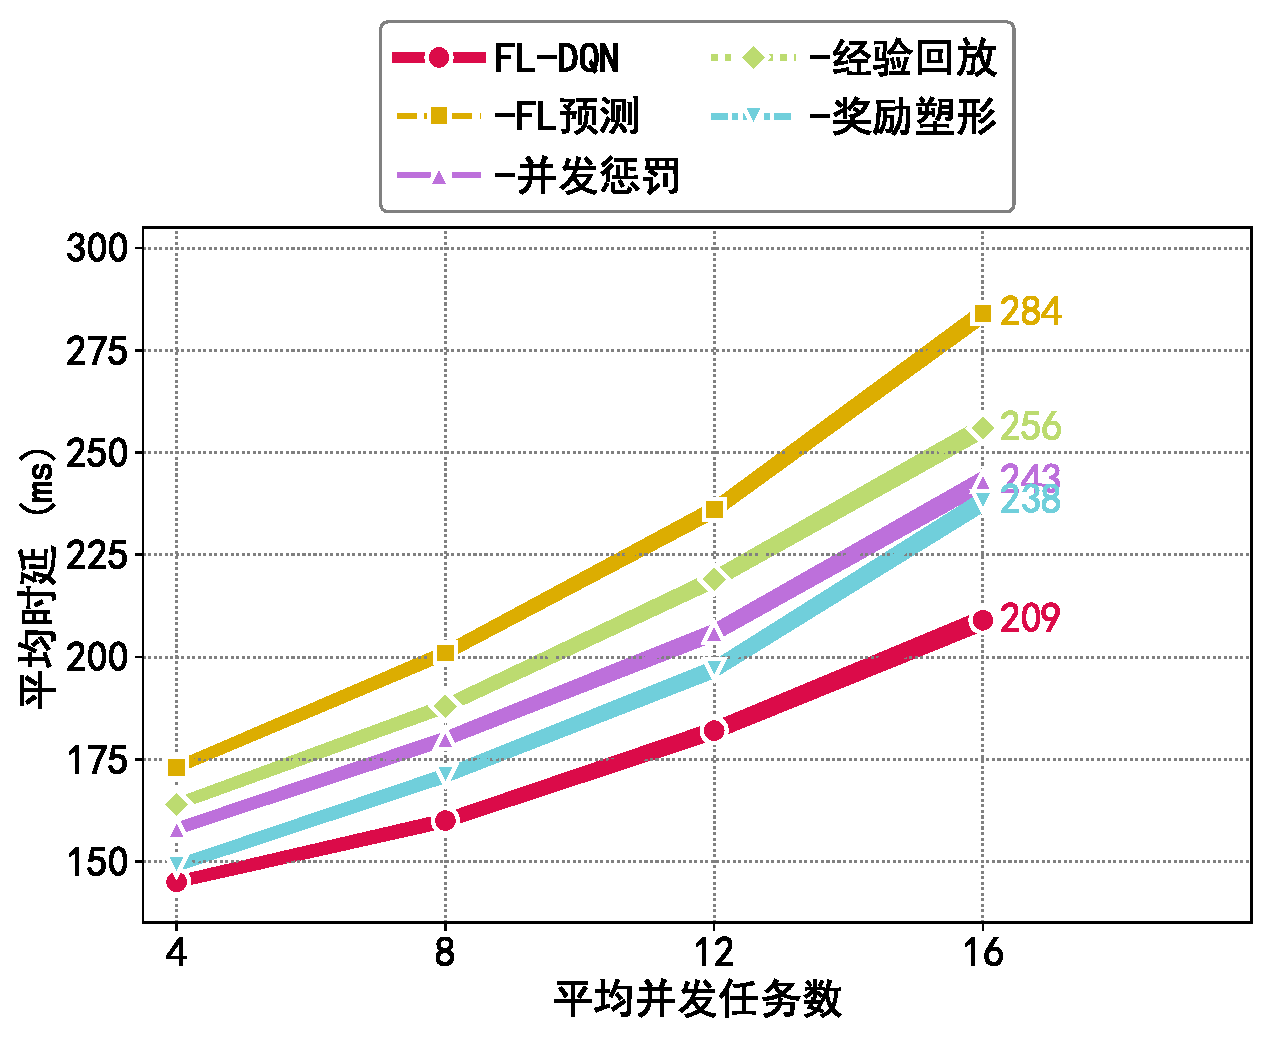
\includegraphics[width=\linewidth]{chapter4_5_fldqn_package/figures/fig4_9_a_avg_delay_cn.eps}
        \caption{平均时延随并发度变化}
    \end{subfigure}
    \hfill
    \begin{subfigure}[t]{0.48\textwidth}
        \centering
        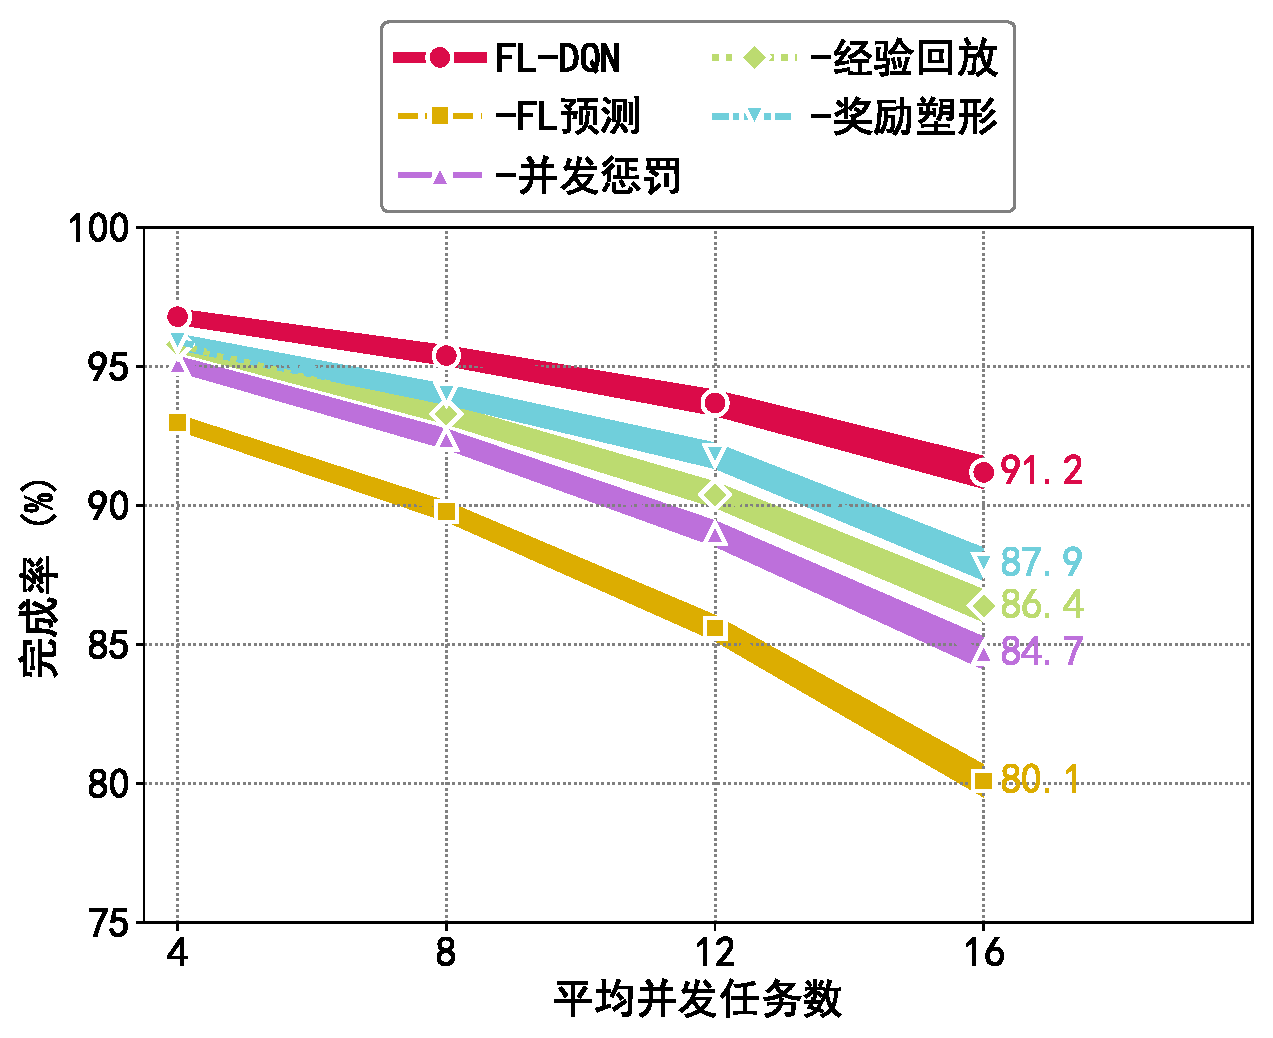
\includegraphics[width=\linewidth]{chapter4_5_fldqn_package/figures/fig4_9_b_sla_cn.eps}
        \caption{SLA 完成率随并发度变化}
    \end{subfigure}
    \caption{消融实验结果}
    \label{fig:ch5_ablation_results_ab}
\end{figure}

\begin{figure}[H]
    \centering
    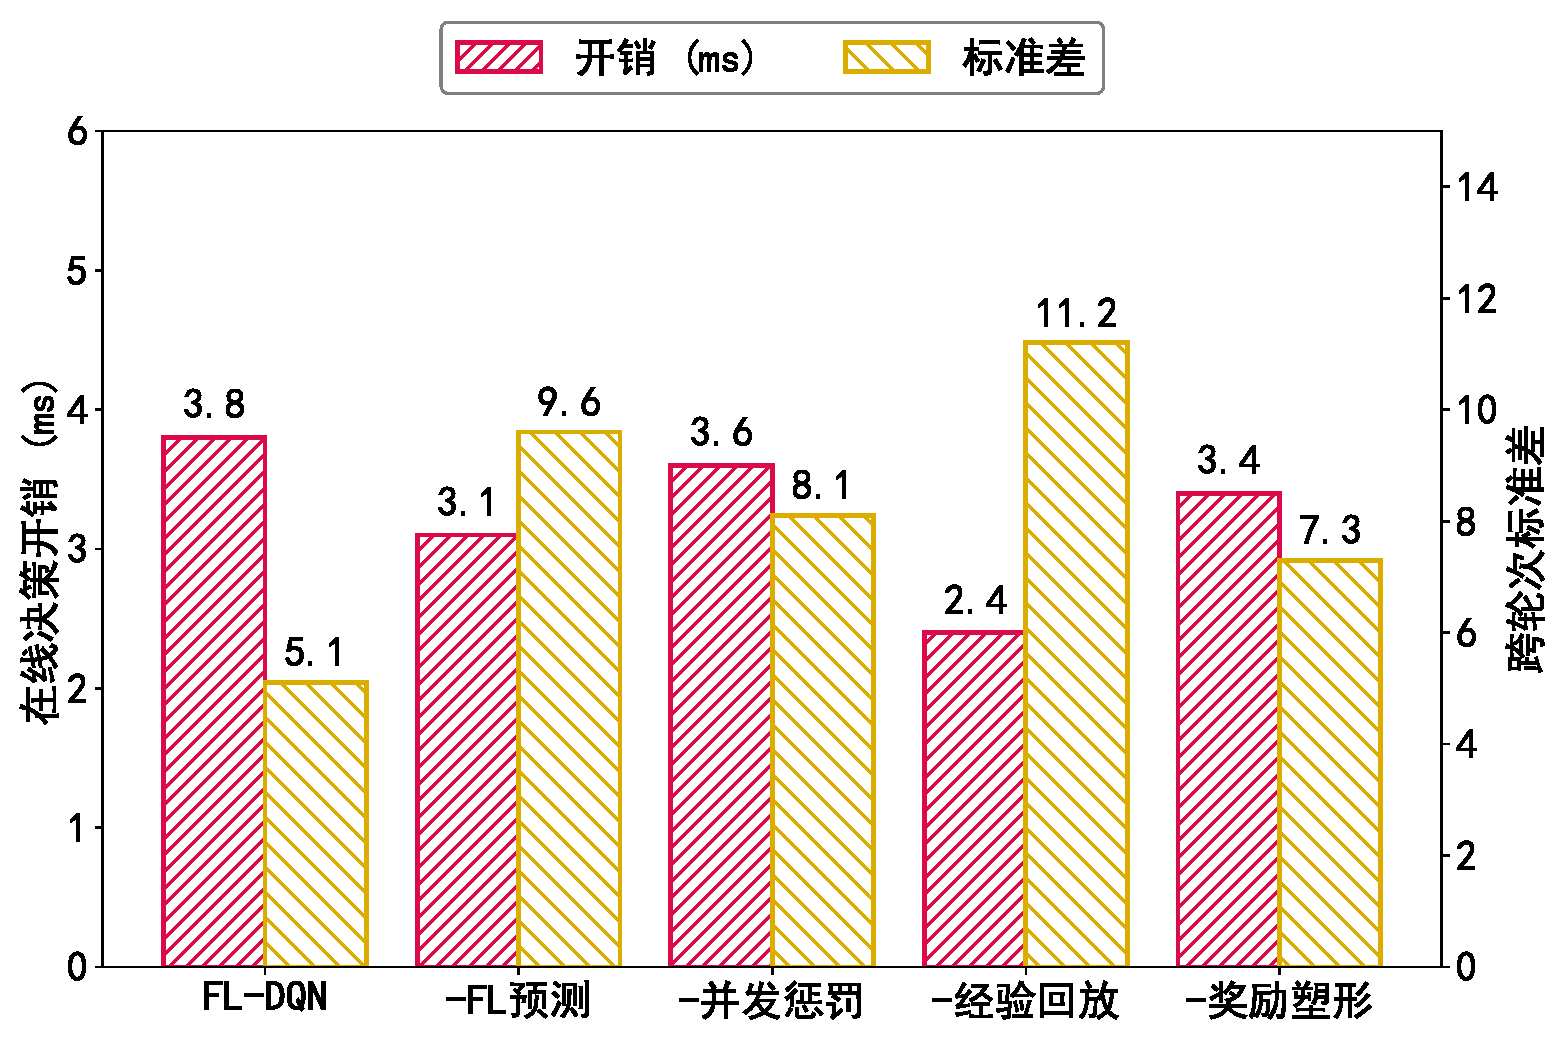
\includegraphics[width=0.76\textwidth]{chapter4_5_fldqn_package/figures/fig4_9_c_overhead_variance_cn.eps}
    \caption{在线决策开销与跨轮次波动联合对比}
    \label{fig:ch5_ablation_results_c}
\end{figure}

平均时延方面，图~\ref{fig:ch5_ablation_results_ab}（a） 显示，完整 FL-DQN 在所有并发水平下都最低；移除 FL 预测模块后时延显著上升，且并发越高、劣化越明显——预测模块正是性能优势的核心来源，缺少先验后 DQN 只能依靠当前观测状态和链上扩展摘要做反应式决策，高并发下更容易产生错误卸载。移除并发惩罚项时延也有上升，但幅度小于移除 FL 预测：并发惩罚负责强化拥塞规避偏好，预测模块决定了策略是否拥有风险前瞻能力，二者所处的位置不同。

SLA 完成率方面，图~\ref{fig:ch5_ablation_results_ab}（b） 显示，完整 FL-DQN 始终最高，并发增强时下降也最平缓。移除 FL 预测后完成率下降最明显，缺少并发开销估计直接影响任务能否在时延阈值内完成；移除并发惩罚同样把完成率压低，仅将预测值作为状态输入并不足以完全引导策略规避拥塞，还需在奖励中显式体现并发开销代价，让智能体在训练中形成对高风险动作的惩罚记忆。

在线开销与跨轮次波动方面，图~\ref{fig:ch5_ablation_results_c} 反映了“效率--稳定性”维度。完整 FL-DQN 的在线开销略高于移除 FL 预测或经验回放的简化版本——决策前需调用预测模型并完成 DQN 动作价值计算——但仍处于毫秒级，能够满足节点侧实时决策需求。与此同时，它的跨轮次标准差最低，多次独立运行下表现更稳定。移除经验回放后在线开销最低，代价却是跨轮次波动显著放大；移除 FL 预测后波动同样明显增大，缺乏稳定的风险先验会削弱策略一致性。完整方法在“决策效率--训练稳定性”之间取得了更优的综合折中。

综合三组结果，FL 预测模块决定了策略的风险前瞻能力，是降低高并发时延、维持 SLA 完成率的关键；并发惩罚项强化了对拥塞节点的规避，让预测信息更直接地转化为优化目标；经验回放主要降低跨轮次波动；奖励塑形改善收敛方向和任务完成质量。FL-DQN 的性能提升不是单个模块的堆叠效果，而是预测先验、奖励约束和强化学习稳定机制相互协同的产物。


\subsection{鲁棒性与敏感性分析}
\label{subsec:ch5_robustness_results}

仅靠平均时延或完成率不足以判断方法是否可部署。天基网络链路窗口有限、链上摘要有确认延迟，节点状态难免陈旧；可部署的卸载策略还需要具备可解释的动作选择行为，并在效率、能耗与节点均衡之间取得合理折中。下面从摘要陈旧性敏感性、动作选择偏好、效率--公平性折中三个角度展开分析，结果见图~\ref{fig:ch5_robustness_action_preference} 与图~\ref{fig:ch5_multi_objective_tradeoff}。

\begin{figure}[H]
    \centering
    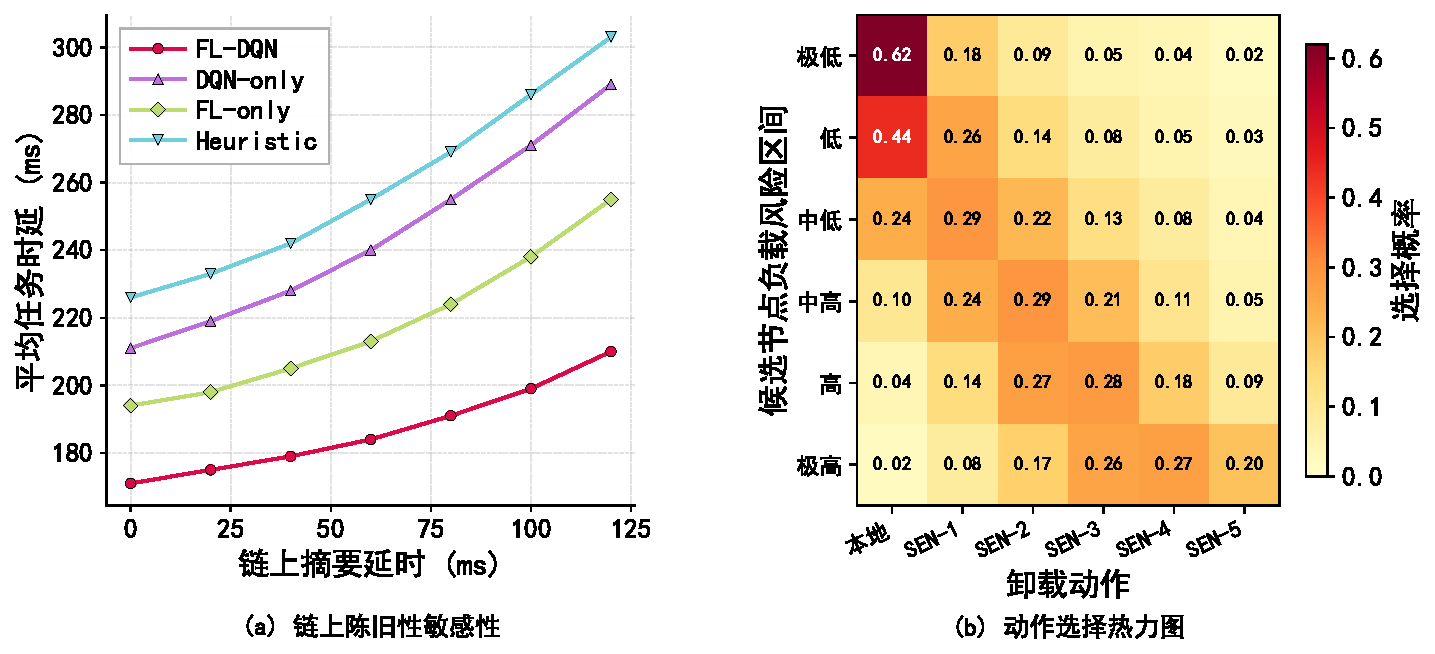
\includegraphics[width=0.88\textwidth]{images/4-new-8-ab.pdf}
    \caption{鲁棒性与动作偏好结果}
    \label{fig:ch5_robustness_action_preference}
\end{figure}

\begin{figure}[H]
    \centering
    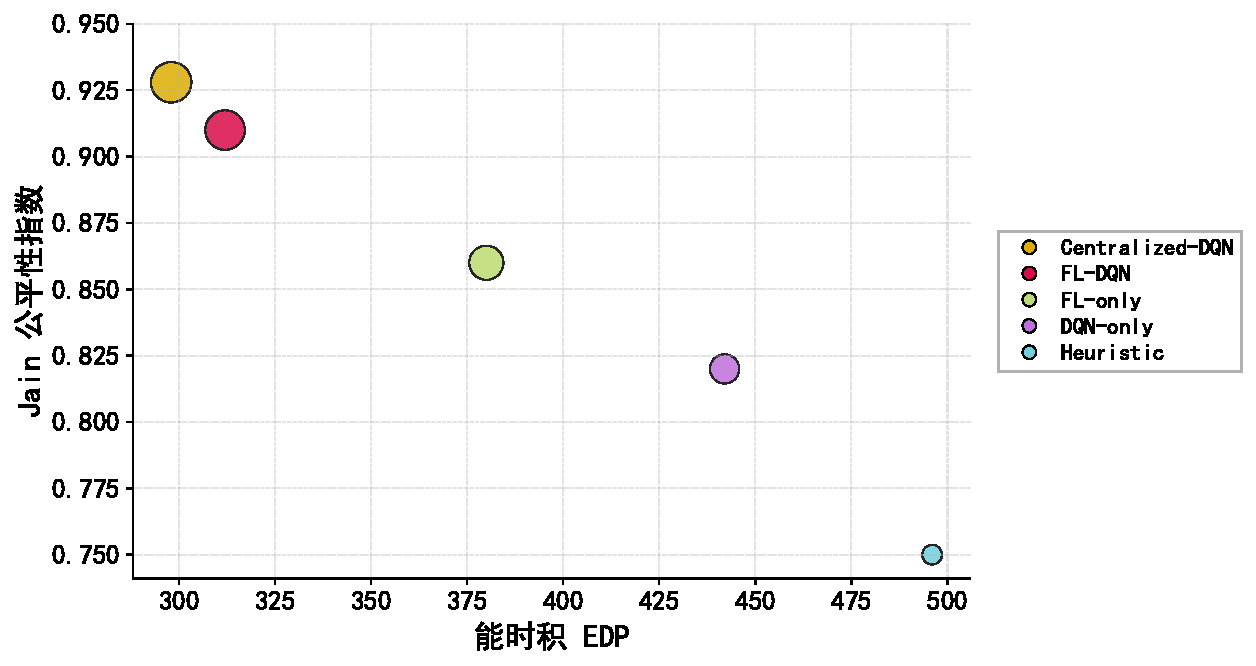
\includegraphics[width=0.72\textwidth]{images/4-new-8-c.pdf}
    \caption{多目标折中结果}
    \label{fig:ch5_multi_objective_tradeoff}
\end{figure}

图~\ref{fig:ch5_robustness_action_preference}（a） 显示，摘要延迟增加时，所有方法的平均时延都在上升——摘要越陈旧，节点负载状态偏离真实运行状态的概率越高，错误卸载也随之增多。但 FL-DQN 的退化幅度明显小于其余方法。这是因为它并不完全依赖链上摘要：本地实时观测与联邦预测模型对状态陈旧性形成了一定补偿，链上摘要无法准确反映当前节点状态时，预测模块仍能基于历史负载模式与并发环境特征估计潜在风险。

图~\ref{fig:ch5_robustness_action_preference}（b） 的动作选择热力图通过策略收敛后测试集中的动作选择频次按风险区间归一化得到。负载风险较低时，策略偏好本地执行或风险较低的候选边缘节点；候选节点负载风险升高后，动作选择逐步向其他节点分散，智能体会根据风险变化动态调整卸载目标，而不是长期锁定某个高性能节点。FL-DQN 学到的不是“选当前负载最低的节点”这种简单规则，而是结合任务属性、链上扩展摘要和并发开销预测的自适应卸载行为。

图~\ref{fig:ch5_multi_objective_tradeoff} 展示了 EDP 与 Jain 公平性指数之间的折中关系，气泡大小表示任务完成率。EDP 越低，时延--能耗的综合效率越好；Jain 指数越高，任务在不同节点之间分配越均衡。Centralized-DQN 凭借理想全局状态在两项指标上均表现较好，但全局实时信息假设让它的实际部署难度也较高；FL-DQN 在 EDP 与公平性之间取得了较优折中，公平性虽略低于集中式上界，仍明显优于 DQN-only、FL-only 和 Heuristic，并保持较高的任务完成率。Heuristic 和 DQN-only 更容易把任务集中到少数表面负载较低的节点，公平性因而下降，能时积也增大。

放在一起看，FL-DQN 的优势不仅体现在平均性能上，也体现在对链上摘要滞后的适应能力、动作选择行为的合理性以及多目标折中能力上——这与天基分布式计算“信息不完全、状态存在滞后、节点负载动态变化”的部署现实更契合。

\subsection{本节小结}
\label{subsec:ch5_exp_summary}

围绕并发感知任务卸载方法的有效性，本节做了分层实验验证。聚类式联邦学习在不集中上传原始日志的前提下能够学到候选节点的并发开销变化规律，并在 Non-IID 环境下保持稳定的预测精度与收敛性；把预测值及其不确定性引入 DQN 后，节点侧策略在平均时延、吞吐量、SLA 完成率和 P99 尾时延等指标上都优于分布式基线方法，中高并发下尤为突出。鲁棒性分析显示 FL-DQN 在链上摘要陈旧时性能退化更平缓，动作选择也符合风险变化规律；消融实验进一步明确了各模块的不同贡献。

实验整体表明，本文所提的 FL-DQN 方法在隐私受限、状态滞后和负载异构的天基分布式计算环境中，能够把联邦学习得到的并发开销预测有效转化为节点侧实时卸载决策的收益，在时延、吞吐量、完成率、尾部稳定性和负载均衡之间取得更合理的折中。

\section{本章小结}
\label{sec:ch5_conclusion}

本章围绕天基网络任务层实时卸载问题，提出了面向并发开销的“联邦预测 + DQN 决策”方法。与第\ref{chap:ch4_system_resource_allocation}章面向较长时间尺度的系统层可信协同不同，本章进一步聚焦节点侧，以单任务到达瞬间的快速动作选择为核心，处理链上摘要滞后、隐私受限、负载动态变化和并发资源竞争等问题，将系统层形成的候选约束、信誉上下文和可信状态基础转化为任务层实时执行能力。

方法层面，本章先从任务层视角统一了时延、能耗与并发开销的代价表达，并给出了并发开销的形式化定义与可计算近似；为应对节点本地日志难以集中上传且样本高度异构的问题，本章采用分层聚类联邦学习框架实现预测模型的隐私友好训练；预测值及其不确定性被显式纳入 DQN 状态空间，并通过并发代价约束、不确定性惩罚和负载均衡惩罚作用于奖励反馈，使卸载策略具备对潜在并发开销的前瞻感知能力。在中等并发工作点 $\bar{k}=8$ 下，FL-DQN 相比 DQN-only 的平均任务时延下降约 $15.3\%$、P99 时延下降约 $22.8\%$、吞吐量提升约 $18.2\%$、SLA 完成率提高约 $6.2$ 个百分点；高并发工作点 $\bar{k}=12$ 下，优势继续扩大，链上摘要滞后条件下也保持着更平缓的退化趋势。

这些结果验证了三点判断：并发开销是影响天基任务级卸载质量的关键隐藏变量，不能被平均负载简单替代；聚类式联邦学习能够在不上传原始数据的前提下有效建模这一变量，为节点侧决策提供风险先验；将预测先验与强化学习决策深度耦合，可以显著增强策略在信息不完全与高并发场景下的鲁棒性。结合第\ref{chap:ch3_unified_model}章的统一建模与可信状态刻画，以及第\ref{chap:ch4_system_resource_allocation}章的系统层可信协同机制，本章在任务层给出了面向单任务到达瞬间的实时决策方法，使全文形成了从统一建模、系统层协同到任务层执行的跨层方法链，也为后续讨论跨层联合优化、多智能体协同决策或星地协同边缘智能等方向留出了延伸空间。

